\chapter{OpenCAL-CLUST - The distributed memory implementation of OpenCAL}
\label{ch:opencal_cluster}
\dictum[Italo Calvino]{ In reality the space in which we moved was all
	battlemented and perforated, with spires and pinnacles which spread out on every side, with cupolas and balustrades and peristyles, with rose windows, with double- and triplearched fenestrations, and while we felt we were plunging straight down, in reality we were racing along the edge of moldings and invisible friezes, like ants who, crossing a city, follow itineraries traced not on the street cobbles but along walls and ceilings and
	cornices and chandeliers. Now if I say city it amounts to suggesting figures that are, in
	some way, regular, with right angles and symmetrical proportions, whereas instead, we
	should always bear in mind how space breaks up around every cherry tree and every leaf
	of every bough that moves in the wind, and at every indentation of the edge of every leaf,
	and also it forms along every vein of the leaf, and on the network of veins inside the leaf,
	and on the piercings made every moment by the riddling arrows of light, all printed in
	negative in the dough of the void, so that there is nothing now that does not leave its
	print, every possible print of every possible thing, and together every transformation of
	these prints, instant by instant, so the pimple growing on a caliph's nose or the soap
	bubble resting on a laundress's bosom changes the general form of space in all its
	dimensions.}%
\vskip 1em


\lettrine[lines=4]{F}{or} most problems in physics and engineering there is a huge demand for improving the time needed to solve a certain problem. For instance, some numerical meteorological models are so complex that even executed on powerful computers the execution time would be so long that by the time the results are available the prediction would be of no practical use.
But speed is not the only important key aspect in scientific computing.
Sometimes, the accuracy of a solution needs to be improved and that usually translates to a bigger and denser discretization of the problem.
It is clear that in order to overcome these limitations more computing power needs to be employed. 
%\section{Introduction}

Nowadays, computing systems are often equipped with more than one GPU.
From high-end workstations, that are able to accommodate up to 8 GPUs or more on the same motherboards to large clusters, that are usually composed of several computing nodes (see Figure \ref{fig:distribuiteMemory} and Section \ref{sec:flynn_tax} at page \pageref{fig:distribuiteMemory} and \pageref{sec:flynn_tax} respectively) each of them equipped with one or more accelerators possibly made by different manufacturers and with different underlying architecture.
Programming distributed memory machines is complex especially for non-HPC computer scientist because of the intrinsic complexity introduced by the parallelism and because of the hardware heterogeneousness, and this is especially true since large clusters are equipped with several accelerators.
However it is important to fully and effectively utilize such computing power, especially since having multiple GPUs per node improves the ratio performance over Watt and price over Watt.
For these reasons, multi-GPU programming is becoming more and more important.

Unfortunately, neither \textsc{CUDA} or \textsc{OpenCL} supports natively a multi-GPU model.
The model they support is based on a \textit{single core}-\textit{single GPU} relationship and works really well for tasks that are independent one from the other.
On the other hand, the aforementioned model makes things more difficult when a task needs to have several GPUs cooperate in some way in order to solve a problem instance.
As an example of an application of the supported model, the \textsc{BOINC} application \cite{anderson:2004} allows a user to donate computing power and time to solve relevant problems.
In a multi-GPU environment, it works spawning $N$ independent tasks and each of them is scheduled on one of the $N$ available GPUs.
When a task is finished, the application simply requests another task to the central server, the \textit{task dispatcher}.
No cooperation or communication is required between the GPUs as the tasks to be solved is self-contained, meaning that it does not need any external input or information to be fully completed.
An example of the unsupported model, consider the Lattice Boltzmann (LB) \cite{McNamara&Zanetti-1988} \cite{Aidun2010439} \cite{Higuera&Jimenez-1989} method on a domain that is decomposed along one axis, let's say the $x$ axis, as depicted in Figure \ref{fig:multigpu_domain_decomposition}, so that each GPU is responsible for a subset of the whole mesh.
Computation for a grid point that lies on the boundary of the domain portion assigned to the GPU $2$ needs information about neighboring points that are stored on different GPUs ($1$ and $3$ in this case). As a consequence, 
communication of such boundary points between the two devices is required.

\section{OpenCAL-CLUST}
This chapter describes the distributed memory version of \texttt{OpenCAL}, \texttt{OpenCAL-CLUST}, which has been designed to take advantage of the modern multi-GPU capabilities of multi-node systems. This makes \texttt{OpenCAL} applications deployable on a variety of computer architectures, from a single CPU workstation to large heterogeneous clusters. 
Section \ref{sec:run_configuration} starts by describing the \textit{configuration file} that is used to dispatch data and computation across the machine. Sections 
\ref{sec:domain_decomposition} and \ref{sec:opencal_cluster_implementation}  outline the adopted parallelization and domain decomposition strategies and introduce a set API and number of examples that show how \texttt{OpenCAL} can be used to code distributed memory applications. Finally, Section \ref{sec:perfomance} discusses performance and tests.
  \begin{figure}
    \begin{center}
        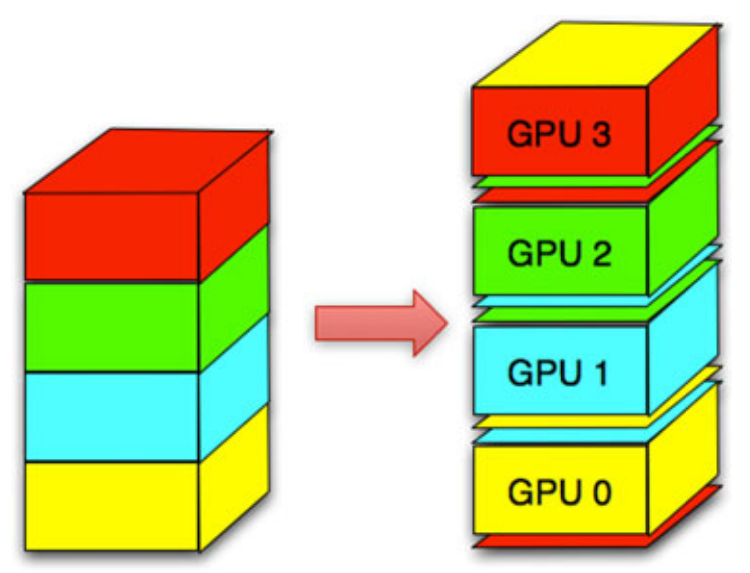
\includegraphics[width=0.67\textwidth]{./images/opencal/multigpu_domain_decomposition.png}
        \caption{Domain decomposition along one axis.}
        \label{fig:multigpu_domain_decomposition}
    \end{center}
\end{figure}



\subsection{Run Configuration}
\label{sec:run_configuration}
Each \texttt{OpenCAL-CLUST}  application is attached with a running configuration that is provided by the user or the programmer and describes both which computational resources are going to be used during the execution and how the domain is decomposed among them.
The running configuration is provided as a plain text file whose syntax and structure are described in Listing \ref{code:file_syntax}.


\captionsetup[table]{name=Listing}
\begin{table}
\renewcommand{\arraystretch}{1} %<- modify value to suit your needs
\centering
\small
\begin{tabular}{m{0.21\linewidth}| m{0.7\linewidth}}
    \toprule
\setlength\extrarowheight{-3em}
    \textsc{domain size}  & 
    \begin{verbatim}
        DIM_1 DIM_2 ... DIM_N
    \end{verbatim}
    \tabularnewline
    %row------------------------
    \textsc{number of nodes}  & 
    \begin{verbatim}
        NUMBER OF NODES
    \end{verbatim}
        %row------------------------
    \tabularnewline
    \midrule
     \textsc{ip node 1}   & 
    \begin{verbatim}
        IP_NODE_1 NUM_GPU_NODE_1
    \end{verbatim}
    %row------------------------
    \tabularnewline
     \textsc{Device List Node $1$}  & 
    \begin{verbatim}
        PLATFORM_NUMBER_1 DEVICE_NUMBER_1 LOAD_1_1
        PLATFORM_NUMBER_1 DEVICE_NUMBER_2 LOAD_1_2
                 ...
        PLATFORM_NUMBER_1 DEVICE_NUMBER_K1 LOAD_1_K1_1
        PLATFORM_NUMBER_2 DEVICE_NUMBER_1  LOAD_2_1
                 ...
    PLATFORM_NUMBER_2 DEVICE_NUMBER_K2 LOAD_2_K1_2
                 ...
    PLATFORM_NUMBER_M1 DEVICE_NUMBER_KM LOAD_M1_K1_M1
    \end{verbatim}
    \tabularnewline
\midrule


     \textsc{ip node 2}   & 
\begin{verbatim}
IP_NODE_2 NUM_GPU_NODE_2
\end{verbatim}
%row------------------------
\tabularnewline
\textsc{Device List Node 2}  & 
\begin{verbatim}
PLATFORM_NUMBER_1 DEVICE_NUMBER_1 LOAD_1_1
PLATFORM_NUMBER_1 DEVICE_NUMBER_2 LOAD_1_2
                 ...
PLATFORM_NUMBER_1 DEVICE_NUMBER_K2_1 LOAD_1_K2_1
PLATFORM_NUMBER_2 DEVICE_NUMBER_1  LOAD_2_1
                 ...
PLATFORM_NUMBER_2 DEVICE_NUMBER_K2 LOAD_2_K2_2
                 ...
PLATFORM_NUMBER_M2 DEVICE_NUMBER_K2_M2 LOAD_M1_K2_M2
\end{verbatim}
\tabularnewline
\midrule
\vspace{-1em}
\centering \scalebox{2.0}{  {$\vdots $} }&\centering \scalebox{2.0}{  {$\vdots $} }\\ 

\tabularnewline
\midrule


\textsc{ip node $N$}   & 
\begin{verbatim}
IP_NODE_N NUM_GPU_NODE_N
\end{verbatim}
%row------------------------
\tabularnewline
\textsc{Device List Node N}  & 
\begin{verbatim}
PLATFORM_NUMBER_1 DEVICE_NUMBER_1 LOAD_1_1
PLATFORM_NUMBER_1 DEVICE_NUMBER_2 LOAD_1_2
                 ...
PLATFORM_NUMBER_1 DEVICE_NUMBER_KN_1 LOAD_1_KN_1
PLATFORM_NUMBER_2 DEVICE_NUMBER_1  LOAD_2_1
                 ...
PLATFORM_NUMBER_2 DEVICE_NUMBER_KN_2 LOAD_2_KN_2
                 ...
PLATFORM_NUMBER_MN DEVICE_NUMBER_KN_MN LOAD_M1_KN_MN
\end{verbatim}
\\ \tabularnewline
\bottomrule
        
\end{tabular}
\caption[File Format for the domain decomposition of a \texttt{OpenCAL-CLUST} application.]{File Format for the domain decomposition of a \texttt{OpenCAL-CLUST} application. It describes the size of the domain and the machine on which the model is executed. Note that for each node of the cluster, the IP address and a list of devices is listed. Each device is identified, \textit{\`a la} \textsc{OpenCL}, by platform and device number (within the platform).}
\label{code:file_syntax}
\end{table}
%table name back to normal
\captionsetup[table]{name=Table}

The configuration file starts with two lines describing:
\begin{enumerate}
    \item The size of the domain along each of the dimensions as a list of positive integers.
    \item The number $N$ of computational nodes, each described and identified uniquely by its IP address.
\end{enumerate}
$N$ descriptions of nodes follow.
A node $i$, $1 \leq i \leq N$ is described by a line containing its IP address $IP_i$ and the number of devices (installed and available on that node) $NUM\_GPU\_NODE_i$ to be utilized.
$NUM\_GPU\_NODE_i$ lines follow, each containing the definition of the devices within node $i$ and its workload. 

A device is identified by its \textbf{platform number} $PLATFORM\_NUMBER_p$, $1 \leq p \leq M_i$, where $M_i$ is the number of the platforms on node $i$, a \textbf{device number within the platform} $DEVICE\_NUMBER_l$ ($l$ relative to the platform). A \textbf{load} parameter for the device $d$, $LOAD^i_{(p,d)}$ describing the amount of work assigned (portion of the domain) to that device.

Eventually, the list of devices within a node can be arbitrarily ordered.



\subsection{Domain Decomposition}
\label{sec:domain_decomposition}
In this preliminary work, the general strategy for dividing work among the available nodes and devices is to decompose the domain along the first dimension listed in the run configuration. The configuration file has to correctly describe a $1D$ decomposition along the first dimension of the domain. This means that the following has to be always true:
\[
\sum_i^N \sum_p^{M_i} \sum_d^{K_p} LOAD^i_{(p,d)} = DIM\_1
\]
i.e. the sum of the loads has to match the size of the first dimension of the domain exactly. This ensures that the whole domain is assigned to some device on a node.

The decomposition follows the order in which nodes and devices are listed in the configuration file. Subsequent portions of not yet assigned portions of the domain are assigned to subsequent (with the respect to the order in which they appear in the file) devices. The size of such portion is described by the device load parameter.

 In order to show how decomposition works, consider the configuration file in Listing \ref{code:configuration_file_example}.
\lstset{
     caption={Configuration file example. Size of the domain is $16384 \times 16384$, scattered along the first dimension among $2$ nodes and $5$ device overall.}, 
     label={code:configuration_file_example}, 
     basicstyle=\footnotesize\ttfamily,
     keywordstyle=\color{blue}\ttfamily,
     stringstyle=\color{red}\ttfamily,
     commentstyle=\color{green}\ttfamily,
     backgroundcolor=\color{light-gray}
     }
 \begin{minipage}{\linewidth}
\begin{lstlisting}
16384 16384
2
192.168.1.111 2  
0 0 4096
0 1 4099
192.168.1.222 3
0 0 1200
1 0 3200
1 1 3792
\end{lstlisting}
\end{minipage}
which defines a $2D$ domain of size $2^{{14} \times 2^{{14}} = 2^{28}}$ points.
The domain is scattered along the first dimension, $x$, among 2 nodes and 5 devices, in the following manner:
\begin{itemize}
    \item $0 \leq x < 4096 \longmapsto$  device $(0,0)$ running at node $192.168.1.111$.
    \item  $4096 \leq x < 4096+4099$ go to device $(0,1)$ running at node $192.168.1.111$.
    
    \item  $4096+4096\leq x < 1200+4096+4096 \longmapsto$  device $(0,0)$ running at node $192.168.1.222$.
    \item  $1200+4096+4096\leq x < 3200+1200+4096+4096 \longmapsto$  device $(1,0)$ running at node $192.168.1.222$.
    \item  $3200+1200+4096+4096\leq x < 3792+3200+1200+4096+4096 \longmapsto$  device $(1,1)$ running at node $192.168.1.222$.
\end{itemize}



Generally speaking, using the decomposition described in section \ref{sec:domain_decomposition}, when $N$ devices are involved, GPU $i$ needs to know, for the update of the grid points within the boundaries of its subdomain, the value of substates of the neighboring subdomains belonging to different devices (that can be possibly located on different nodes). 
At each iteration, it must perform all the operations depicted in Figures \ref{fig:communication_scheme} and \ref{fig:multigpu_naive_exchange} (assuming periodic boundary conditions for the sake of simplicity).
\begin{figure}[H]
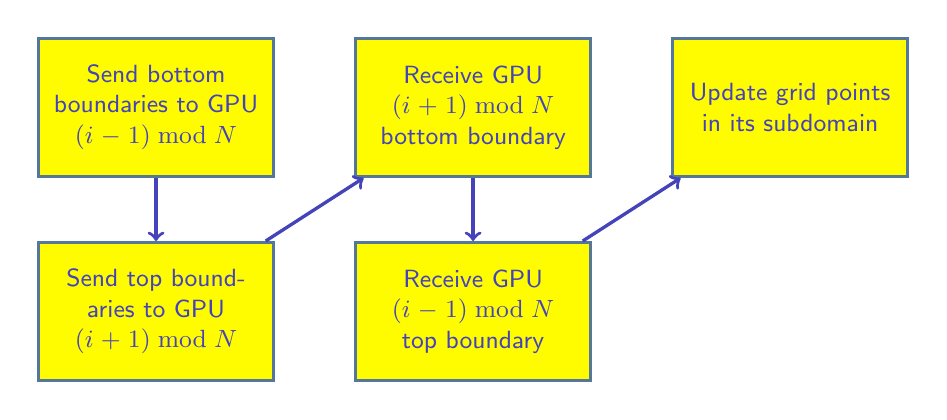
\begin{tikzpicture}
\definecolor{blue1}{HTML}{4443ba}
\definecolor{blue2}{HTML}{55779A}
\definecolor{myyellow}{HTML}{fffc00}
\definecolor{myblue}{HTML}{4443ba}
\matrix [column sep=10mm, row sep=8mm, every node/.style={
    shape=rectangle,
    text width=2.75cm,
    minimum height=1.75cm,
    text centered,
    font=\sffamily\small,
    very thick,
    color=myblue,
    draw=blue2,
    fill=myyellow,
}] {
    \node (a1) {Send bottom boundaries to GPU $(i-1)\bmod N$}; &
    \node (a2) {Receive GPU $(i+1)\bmod N$ bottom boundary}; &
    \node (a3) {Update grid points in its subdomain}; \\
    
    \node (b1) {Send top boundaries to GPU $(i+1)\bmod N$}; &    
    \node (b2) {Receive GPU $(i-1)\bmod N$ top boundary}; &
    \\
};
\begin{scope}[->, very thick, blue1]
\draw (a1) -- (b1);
\draw (b1) -- (a2);
\draw (a2) -- (b2);
\draw (b2) -- (a3);
\end{scope}
\end{tikzpicture}
\caption{Communication scheme in a multi-GPU OpenCL application}
\label{fig:communication_scheme}
\end{figure}

%\begin{enumerate}
%    \item send its bottom boundary to the GPU number $(i-1) \bmod N$
%    \item send its top boundary to the GPU number $(i+1) \bmod N$
%    \item receive $(i+1) \bmod N$ bottom boundary
%    \item receive $(i-1) \bmod N$ top boundary
%    \item update grid points belonging to nodes of its subdomain
%\end{enumerate}

\begin{figure}
    \centering
        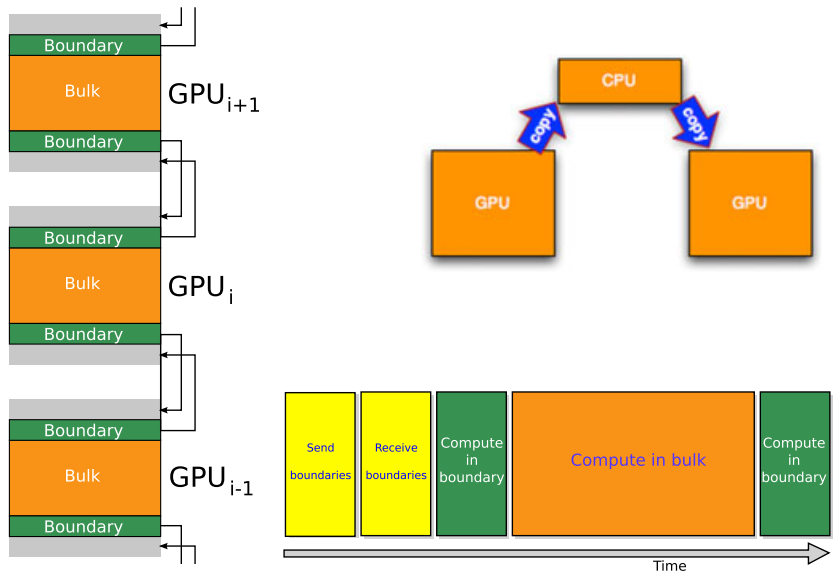
\includegraphics[width=1.0\textwidth]{./images/opencal/multigpu_naive_exchange.png}
        \caption{The adopted multi-GPU computation scheme.}
        \label{fig:multigpu_naive_exchange}
\end{figure}


Note that this approach always requires CPU intervention as the OpenCL device-device memory transfer feature in the current implementation only works between devices that are within the same OpenCL context. This implies that synchronization is also required during the boundary exchange, as depicted in figure \ref{fig:multigpu_naive_exchange}b.
For a communication step to take place, it is necessary to:
\begin{enumerate}
    \item Pack and upload boundary data to the CPU ( device$\,\mapsto\,$host  memory transfer)
    \item If the two GPUs involved in the communications are controlled by different nodes, an extra communication step over the network is performed between the two nodes. This phase is implemented via MPI \cite{mpiStandard:1994} to ensure and guarantee portability and scalability. 
    \item Unpack and upload boundary data to the recipient GPU (host$\,\mapsto\,$device memory transfer).
\end{enumerate}


\section{The \texttt{OpenCAL-CLUST}  Parallel Implementation}
\label{sec:opencal_cluster_implementation}
  In this section, the OpenCL distributed memory and multi-GPU parallel implementation of \texttt{OpenCAL} is described, which allows for the parallel execution on one or more accelerators installed on computing nodes interconnected via network and MPI.
This section describes the difference between OpenCAL-CL and \texttt{OpenCAL-CLUST}  and discusses only the set of the additional API calls that the latter version exposes. 

The programming model adopted by \texttt{OpenCAL-CLUST}  is similar to the other versions of \texttt{OpenCAL} (see Section \ref{ch:opencal}) but it introduces new concepts that mainly reflect the multi-GPU and multinode structure of the target machines.

The main difference is the addition of the \texttt{MultiNode} class (see Listing \ref{code:multinode}).
\lstset{language=[OpenCL]C,frame=tb,
    caption={\texttt{OpenCAL-CLUST} MultiNode Class Declaration}, 
    label={code:multinode}, 
    basicstyle=\footnotesize\ttfamily,
    keywordstyle=\color{blue}\ttfamily,
    stringstyle=\color{red}\ttfamily,
    commentstyle=\color{green}\ttfamily,
    backgroundcolor=\color{light-gray}, 
}
\begin{lstlisting}
template <class Init_Functor,class Finalize_Functor>
class MultiNode{
public:
    Cluster c;
    Init_Functor *init;
    Finalize_Functor *finalize;
        ...
\end{lstlisting}
It manages communications and computations across nodes and across GPUs and must be constructed by all the processes/nodes.

In order to use \texttt{OpenCAL-CLUST}, a valid domain decomposition must be specified, see Section \ref{sec:domain_decomposition} and \ref{sec:run_configuration}.
The Domain Decomposition format described in section \ref{sec:domain_decomposition} is reflected in the \texttt{OpenCAL} implementation with the following classes:
\begin{description}
    \item[\texttt{Device}] described by $4$ non-negative integers, two of which identify the device  within the node (using the OpenCL idiom of platform and device numbers) while the rest describe the portion of the subdomain assigned to the specific device.
    \item[\texttt{Node}] containing an IP address, a integer values describing the portion of subdomain assigned to it and finally, a list of \texttt{Device}s installed on the machine that are used for the computation.
    \item [\texttt{Cluster}] containing a list of \texttt{Node}s that are concurrently used to  execute an \texttt{OpenCAL} application.
\end{description}
Each \texttt{OpenCAL-CLUST}  application necessitates of a \texttt{Cluster} object correctly initialized that can conveniently constructed from a file using the \texttt{calFromClusterFile} function exposed. Given a configuration file, \texttt{calFromClusterFile} parses, validates and finally returns a valid \texttt{Cluster} instance.

The information stored in the \texttt{Cluster} object is then utilized by each MPI process to allocate and to initialize all the listed devices.
The library is designed s.t. each MPI process runs several instances of  OpenCAL-CL (see Section \ref{sec:OpenCAL-CL}), each executing on a different device and on a different portion of the original subdomain.
Note also that, \texttt{OpenCAL-CLUST}  degenerates to OpenCAL-CL when only one none and one device are utilized, and that a multi-GPU single node configuration is obtainable specifying a single node with several devices in the configuration file.

Devices within a node are managed by a \texttt{CALCLMultiGPU} object,  which coordinates them and can be created using the \texttt{calclMultiGPUDef2D} API call. \texttt{CALCLMultiGPU} takes care of storing hooks to a per node's devices and resources as the list of compiled kernels for each device.
It also exposes a number of functions for adding or removing a device from the pool and for boundaries exchange between two devices. 


\subsection{\texttt{Init} and \texttt{finalize} functors}
Listing \ref{code:multinode} shows that the \texttt{MultiNode} object, among others fields, contains a \texttt{Cluster} object and two pointers to functors which type is shown in listing \ref{code:init_finalize_signature}.
\lstset{language=[OpenCL]C,frame=tb,
    caption=\texttt{OpenCAL-CLUST}  init and finalize functor signature, 
    label={code:init_finalize_signature}, 
    basicstyle=\footnotesize\ttfamily,
    keywordstyle=\color{blue}\ttfamily,
    stringstyle=\color{red}\ttfamily,
    commentstyle=\color{green}\ttfamily,
    backgroundcolor=\color{light-gray}, 
}
\begin{lstlisting}
void finalize(struct CALCLMultiGPU*);
void init(struct CALCLMultiGPU*, const Cluster*);
\end{lstlisting}

\texttt{init} and \texttt{finalize} if defined, are executed by each MPI process (Node) at the initialization and finalization phases, respectively.
Their definition is optional. They can be employed to perform operations that are hard to manage automatically on a per-node basis. For example, a certain node might need a particular initialization phase such as module loading for instance. The library can completely hide the initialization and allocation phases, but it is important to note that this behaviour can be changed and manual initialization can be enabled. When it is the case, the init functor can be employed to take care of making sure that each MPI process allocates all of its listed devices with the right resources in order to process the assigned domain. 

Listing \ref{code:init} shows an example of init function that is part of the Opencal Julia Set generator example application shown in section \ref{sec:julia_math} and in listing \ref{code:julia_set}. It shows how manual initialization can be performed from the configuration file. Each nodes access its own list of devices using its MPI rank (lines 3-4)  and add them all to the pool using the \texttt{calclAddDevice} function (lines 7-11).
\lstset{language=[OpenCL]C,frame=tb,
    caption=\texttt{OpenCAL-CLUST}  finalize example code for the Julia Set generator application. It outputs the node's portion of a substate to a file., 
    label=code:init, 
    basicstyle=\footnotesize\ttfamily,
    keywordstyle=\color{blue}\ttfamily,
    stringstyle=\color{red}\ttfamily,
    commentstyle=\color{green}\ttfamily,
    backgroundcolor=\color{light-gray}, 
    numbers=left,numbersep=3pt,, 
    numberstyle=\tiny
}
\begin{lstlisting}
void init(struct CALCLMultiGPU* multigpu, const Cluster* c){
    //add devices from the cluster configuration
    Node mynode = c->nodes[rank];
    auto devices = mynode.devices;
    struct CALCLDeviceManager* calcl_device_manager = calclCreateManager();
    calclSetNumDevice(multigpu, devices.size());
    for (auto& d : devices) {
        calclAddDevice(multigpu, 
            calclGetDevice(calcl_device_manager, d.num_platform, d.num_device),
            d.workload);
    }
    //create the model    
    struct CALModel2D* host_CA =
    calCADef2D(mynode.workload, mynode.columns, CAL_MOORE_NEIGHBORHOOD_2D, CAL_SPACE_TOROIDAL, CAL_NO_OPT);
    //add the substate
    Q_fractal = calAddSubstate2Di(host_CA);
    //gosh  cells radius
    int borderSize = 1;
    calclMultiGPUDef2D(multigpu, host_CA, KERNEL_SRC, KERNEL_INC,
                     borderSize, mynode.devices, c->is_full_exchange());
    calclAddElementaryProcessMultiGPU2D(multigpu,     KERNEL_LIFE_TRANSITION_FUNCTION);
}
\end{lstlisting}
Listing \ref{code:init} shows also that cluster object is used to eventually configure a \texttt{calclMultiGPUDef2D} object (line 19). 
Note that the decomposition along the first dimension of the domain is clear here. A CALModel2D object is created using the node's workload (the number of rows in this case).

The finalize functor is executed, if defined, at the end of the computation at the node level. Listing \ref{code:finalize} shows an example in which the \texttt{finalize} is used to save a per node copy of the grid to a file.
\lstset{language=[OpenCL]C,frame=tb,
    caption=\texttt{OpenCAL-CLUST} init and finalize functor signature, 
    label=code:finalize, 
    basicstyle=\footnotesize\ttfamily,
    keywordstyle=\color{blue}\ttfamily,
    stringstyle=\color{red}\ttfamily,
    commentstyle=\color{green}\ttfamily,
    backgroundcolor=\color{light-gray}, 
    numbers=left,numbersep=3pt,, 
    numberstyle=\tiny\ttfamily\color{gray}
}
\begin{lstlisting}
void finalize(struct CALCLMultiGPU* multigpu){
//for each node, save the substate to a file
std::string fractal_str = "./fractal_portion" + std::to_string(rank)+".txt";
    calSaveSubstate2Di(multigpu->device_models[0]->host_CA, fractal_substate, (char*)fractal_str.c_str());
}
\end{lstlisting}
Note that an implicit MPI barrier is present right before the execution of the \texttt{init} and \texttt{finalize} call.

A MultiNode is used in user code as shown in listing \ref{code:multinode_user_code}
\lstset{language=[OpenCL]C,frame=tb,
    caption=\texttt{OpenCAL-CLUST}  init and finalize functor signature, 
    label={code:multinode_user_code}, 
    basicstyle=\footnotesize\ttfamily,
    keywordstyle=\color{blue}\ttfamily,
    stringstyle=\color{red}\ttfamily,
    commentstyle=\color{green}\ttfamily,
    backgroundcolor=\color{light-gray}, 
}

\begin{lstlisting}
    //Construct a MultiNode object
    MultiNode<decltype(init), decltype(finalize)> mn(cluster, mpi_world_rank, init, finalize);
    //trigger allocation and init execution
    mn.allocateAndInit();
\end{lstlisting}

\subsection{Kernel Side }
Kernel side  API  and \textit{build-in} variables are added. Those additional variables and functions can be used to access and manage boundary cells belonging to neighboring devices, the so call \textit{ghost cells}. Each device keeps an updated copy of neighboring devices boundaries and offers to the programmer the abstraction of a single domain. A \textit{built-in} variable, \texttt{border\_radius} is exposed in the kernel side and can be used, from within the kernel, to retrieve the size of boundaries.


The following sections provides examples of usage of \texttt{OpenCAL-CLUST} . Section \ref{sec:opencal_julia} provides a complete code that generates large \texttt{BMP} images of Julia Sets.
Section \ref{sec:convolutional_filters_example} shows how to apply a Sobel's convolutional filter to a large 2D image.
Section \ref{sec:opencal_cluster_sciddicaT} shows an implementation of \textit{sciddicaT}, described in Section \ref{sec:SciddicaT-naive}. 
\section{\texttt{OpenCAL-CLUST}  High Resolution Julia Set Generation}
\label{sec:opencal_julia}
As a first illustrative example of the usage of \texttt{OpenCAL-CLUST}  this section shows an application which generates high resolution Julia Set images running on an heterogeneous cluster of GPUs.

\subsection{Julia Set}
\label{sec:julia_math}
Julia set fractals are normally generated by initializing a complex number  $z = x + yi$  where  $i2 = -1$  and $x$ and $y$ are image pixel coordinates. Then, $z$ is repeatedly updated using:
\[ 
 z_{n+1} = z_n^2 + c
\]  
where $c$ is a complex constant that gives a specific Julia set (see Figure \ref{fig:julia_set_c}).

\begin{figure}[!htb]

    \minipage{0.32\textwidth}
    \begin{subfigure}{1.0\textwidth}
        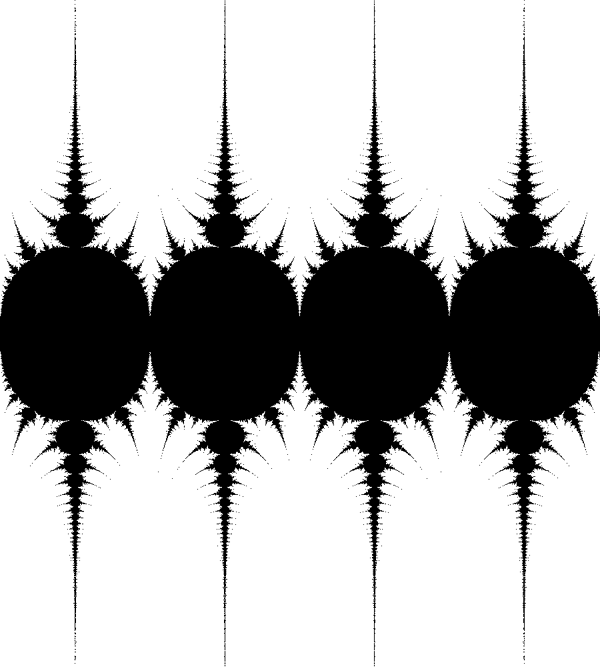
\includegraphics[width=\linewidth]{./images/opencal/julia1.png}
        \label{fig:julia1}
        \caption{$c=1+0i$}
    \end{subfigure}        
    \endminipage\hfill
    \minipage{0.32\textwidth}
    \begin{subfigure}{1.0\textwidth}
        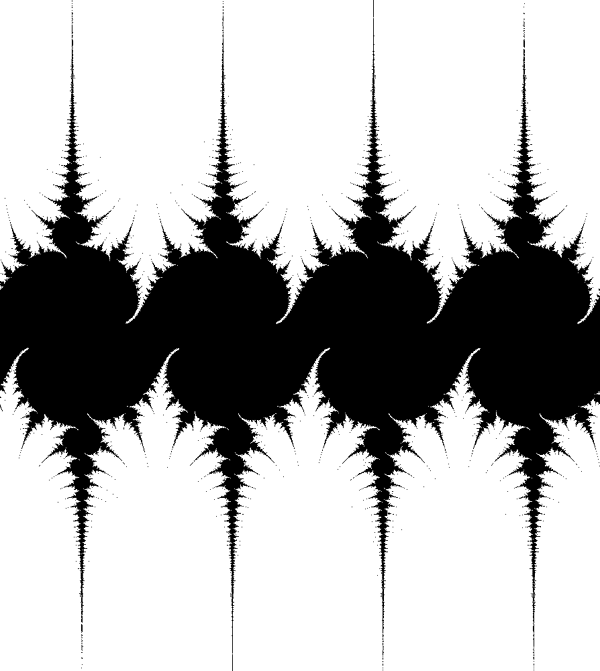
\includegraphics[width=\linewidth]{./images/opencal/julia2.png}
        \label{fig:julia2}
        \caption{$c=1+0.1i$}
    \end{subfigure}
    \endminipage\hfill
    \minipage{0.32\textwidth}%
    \begin{subfigure}{1.0\textwidth}
    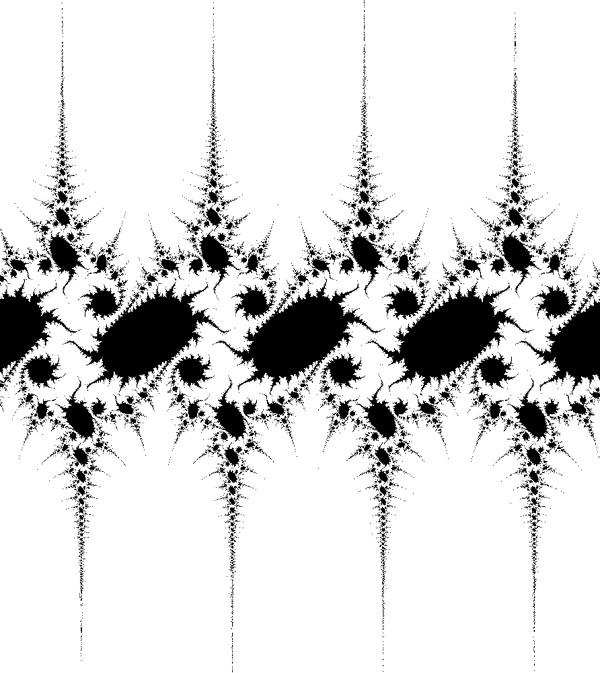
\includegraphics[width=\linewidth]{./images/opencal/julia3.png}
    \label{fig:julia3}
    \caption{$c=1+0.2i$}
\end{subfigure}    
    \endminipage
    \hfill \\ %second row
    \minipage{0.32\textwidth}
        \begin{subfigure}{1.0\textwidth}
        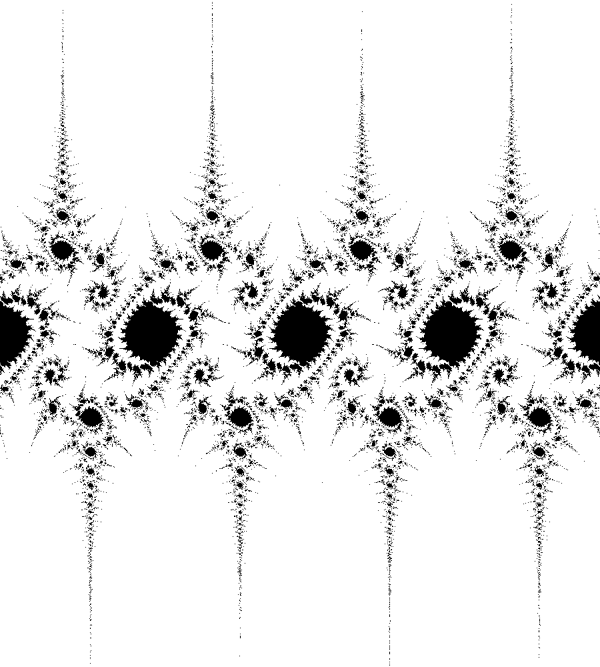
\includegraphics[width=\linewidth]{./images/opencal/julia4.png}
        \label{fig:julia4}
        \caption{$c=1+0.3i$}
    \end{subfigure}
    \endminipage\hfill
    \minipage{0.32\textwidth}
        \begin{subfigure}{1.0\textwidth}
        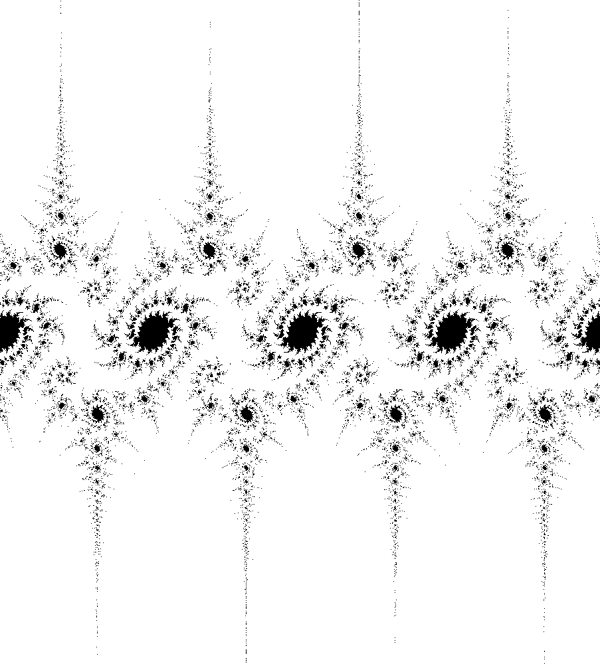
\includegraphics[width=\linewidth]{./images/opencal/julia5.png}
        \label{fig:julia5}
        \caption{$c=1+0.4i$}
    \end{subfigure}
    \endminipage\hfill
    \minipage{0.32\textwidth}%
        \begin{subfigure}{1.0\textwidth}
        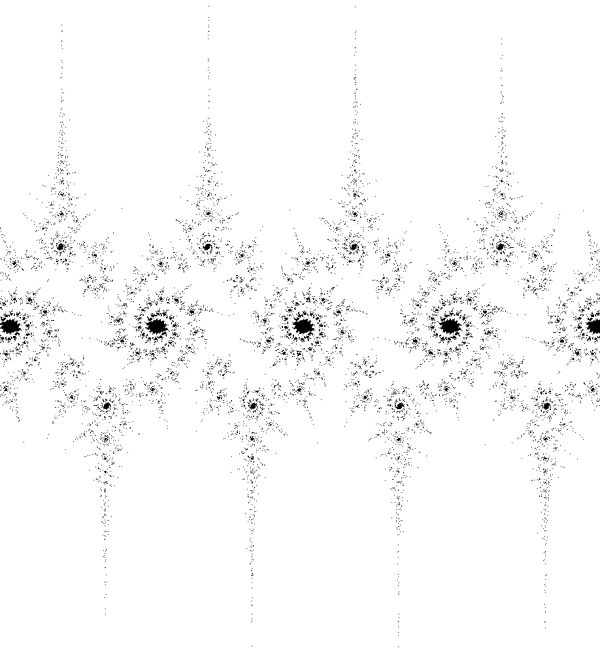
\includegraphics[width=\linewidth]{./images/opencal/julia6.png}
        \label{fig:julia6}
        \caption{$c=1+0.5i$}
    \end{subfigure}
    \endminipage
    
    \caption{6 Examples of Julia sets obtained variating the constant $c$.}
        \label{fig:julia_set_c}
\end{figure}

In the broader sense the exact form of the iterated function may be almost anything of the form $z_{n+1} = f(z_n)$. Interesting sets arises with non-linear functions. Commonly used ones include the following:
\begin{align*}
z_{n+1} &= c\, sin(z_n) & z_{n+1} &= c \,exp(z_n)\\
z_{n+1} &= i\,c\, cos(z_n) &z_{n+1} &= c\, z_n(1-z_n)
\end{align*}

A point is said to be part of the set if after the repeated iteration it does not tend to infinity.
The fractal is created by first mapping each pixel to a rectangular region of the complex plane. Each pixel represents the initial value of $z_0$. The series is computed for each pixel and if it does not diverge to infinity it is drawn in black while, if it doesn't, then a color is chosen depending on the number of iterations taken to diverge. Nevertheless, this convergence or otherwise isn't always obvious and it may take a large number of iterations to resolve and so a decision procedure is required to determine divergence. This typically involves assuming the series tends to infinity as soon as its value exceeds some threshold; if the series has not diverged after a certain number of terms it is similarly assigned to be part of the set. 

\subsection{Julia Sets \texttt{OpenCAL-CLUST}  implementation}
In order to generate the fractal, for each pixel, information regarding how many steps are necessary to diverge is stored in a single integral substate.
In order to compute this value, the iterative process described in Section \ref{sec:julia_math} is implemented in listing \ref{code:julia_set} and is executed once for each pixel of the final image.

As \texttt{OpenCAL} uses OpenCAL-CL, source code and execution is divided in \textit{host} and \textit{device}(kernels), parts ( see Section \ref{sec:OpenCAL-CL}).  

Host side code is shown in listing \ref{code:julia_set_host}. Note that \texttt{init} and \texttt{finalize} functions are omitted since already shown in listings \ref{code:init} and \ref{code:finalize}.
The application takes as an input parameter a configuration file that describes the size and the partitioning of the domain among the nodes and the devices of the cluster. It constructs a \texttt{Cluster} objects out of it using the \texttt{fromClusterFile} function.
The MultiNode class is then created (line 13), and used to allocate  (line 14) and eventually starts the executions (line 17).
\lstset{language=[OpenCL]C,frame=tb,
    caption=\texttt{OpenCAL-CLUST} kernel for the generation of Julia Set., 
    label={code:julia_set_host}, 
    basicstyle=\footnotesize\ttfamily,
    keywordstyle=\color{blue}\ttfamily,
    stringstyle=\color{red}\ttfamily,
    commentstyle=\color{green}\ttfamily,
    backgroundcolor=\color{light-gray}, 
    numbers=left,numbersep=3pt,, 
    numberstyle=\tiny\ttfamily\color{gray}
}
\begin{lstlisting}
#define KERNEL_SRC "~/fractal2D/kernel_fractal2D/source/"
#define KERNEL_INC "~/fractal/kernel_fractal2D/include/"
#define KERNEL_LIFE_TRANSITION_FUNCTION "fractal2D_transitionFunction"

struct CALSubstate2Di *Q_fractal; 
int main(int argc, char** argv){
        //create the cluster file from input parameter path
        string clusterfile;
        clusterfile = parseCommandLineArgs(argc, argv);
        Cluster cluster;
        cluster.fromClusterFile(clusterfile);
        //declare and initialize a multinode object
        MultiNode<decltype(init), decltype(finalize)> mn(cluster, world_rank, init, finalize);
        mn.allocateAndInit();
        //start crunching numbers
        MPI_Barrier(MPI_COMM_WORLD);
        mn.run(STEPS);
        //a barrier and finalize functor are implicitly called here
    return 0;
}

\end{lstlisting}
The \texttt{run} function takes care of splitting the domain and handle communication among the devices transparently. This means that at each iteration the code shown in Listing \ref{code:julia_set} is executed on each device and on each point of the grid assigned to it. Note that in this example, boundaries communication is not required, since no neighboring values are needed in order to compute the value of a pixel.

\lstset{language=[OpenCL]C,frame=tb,
    caption=\texttt{OpenCAL-CLUST} kernel for the generation of Julia Set., 
    label={code:julia_set}, 
    basicstyle=\footnotesize\ttfamily,
    keywordstyle=\color{blue}\ttfamily,
    stringstyle=\color{red}\ttfamily,
    commentstyle=\color{green}\ttfamily,
    backgroundcolor=\color{light-gray}, 
    numbers=left,numbersep=3pt,, 
    numberstyle=\tiny\ttfamily\color{gray}
}
\begin{lstlisting}
typedef double2  cl_complex;

#define DEVICE_Q_fractal (0)
#define MAXITERATIONS (5000)
#define SIZE (16384)
#define moveX (0)
#define moveY (0)
// Maps and zoom a pixel (x,y) to the complex plane
cl_complex convertToComplex(const int x, const int y, const double zoom,
const int DIMX, const int DIMY) {
    double jx = 1.5 * (x - DIMX / 2.0) / (0.5 * zoom * DIMX) + moveX;
    double jy = (y - DIMY / 2.0) / (0.5 * zoom * DIMY) + moveY;
    return (cl_complex)(jx, jy);
}
cl_complex juliaFunctor(const cl_complex p, cl_complex c) {
    const cl_complex c_ipow =
        cl_complex_multiply(&p, &p); 
    return cl_complex_add(&c_ipow, &c);
}
//Returns the number of iteration taken to diverge to infinity 
int evolveComplexPoint(cl_complex p, cl_complex c) {
    int it = 1;
    while (it <= MAXITERATIONS && cl_complex_modulus(&p) <= 10) {
        p = juliaFunctor(p, c);
        it++;
    }
    return it;
}
__kernel void fractal2D_transitionFunction(__CALCL_MODEL_2D) {
    calclThreadCheck2D();
    int i = calclGlobalRow() + borderSize;
    int j = calclGlobalColumn();
    
    const double zoom = 1.0;
    const cl_complex c;    c.x = -0.391;c.y = -0.587;
    
    int global_i = i - borderSize + offset;
    cl_complex p = convertToComplex(global_i, j, zoom, SIZE, SIZE);
    calclSet2Di(MODEL_2D, DEVICE_Q_fractal, i, j, evolveComplexPoint(p, c));
}
\end{lstlisting}


 \begin{figure}[H]
    \begin{center}
        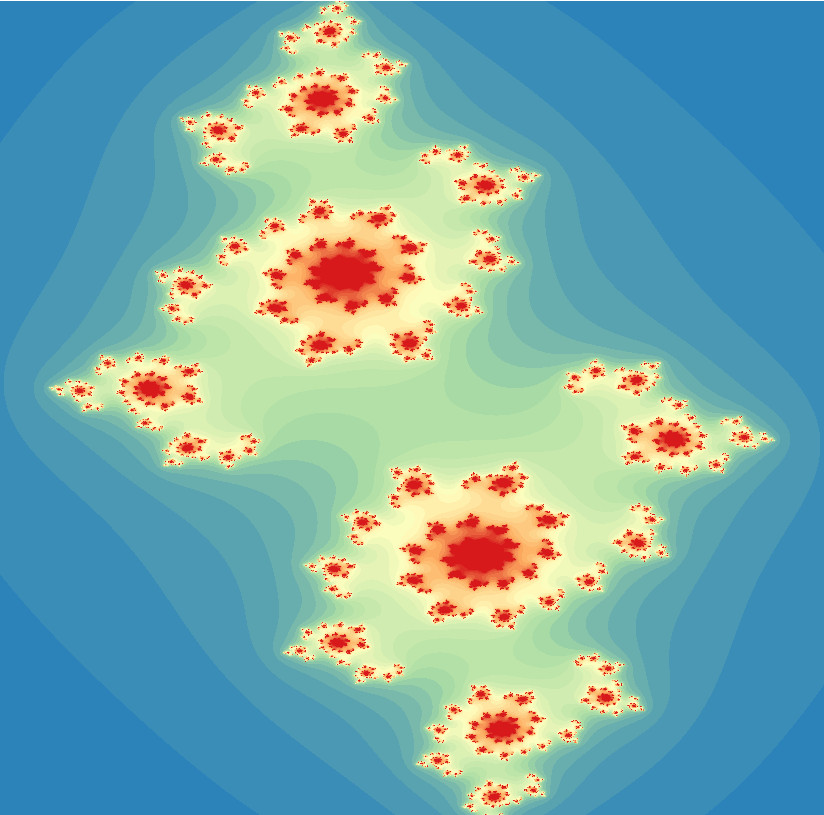
\includegraphics[scale=0.35]{./images/opencal/fractal16k16k}
        \caption[Julia set of size 1.07 GigaPixel generated using \texttt{OpenCAL-CLUST}.]{Julia set of size 1.07 GigaPixel, $\approx 3.22 GB$ in the BMP uncompressed format. It is generated using \texttt{OpenCAL-CLUST} on two \texttt{NVIDIA GTX 980} and rendered on QGIS \cite{QGIS_software} interpreting each point value as color intensity in the spectral color map. Note that the Figure has been subsequently optimized and rescaled for book format.}
        \label{fig:fractal16k16k}
    \end{center}
\end{figure}

\subsection{Convolutional Filters}
\label{sec:convolutional_filters}
The example presented in this section is an application that applies the Sobel convolutional filter on a large 2D image. The code presented can be trivially extended to support any kind of convolutional filter also on a domain with more dimensions. (XXX riferimento a filtri convoluZZionali e Sobel)

 \begin{figure}
    \begin{center}
        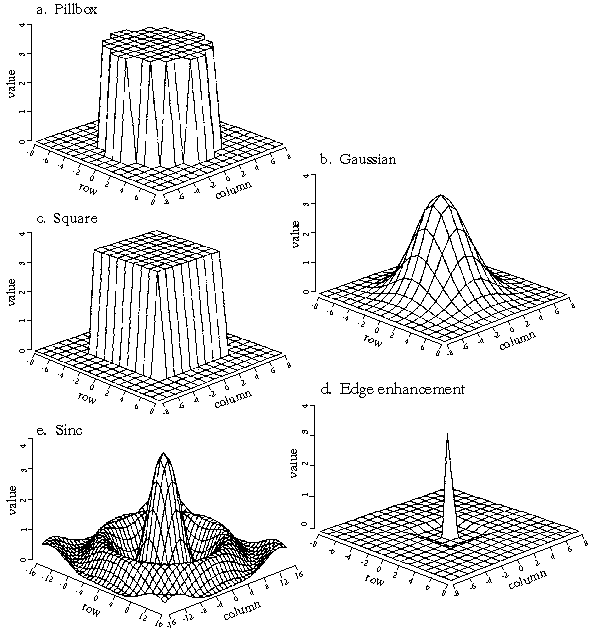
\includegraphics[width=0.72\textwidth]{./images/opencal/kernel_functions}
        \caption[Common point spread functions.]{Common point spread functions. The Pillbox (a), Gaussian (b) and Square (c) are common smoothing, low-pass filters. Edge enhancement (d) is an example of high-pass filter. }
        \label{fig:kernel_functions}
    \end{center}
\end{figure}
Convolution filtering is used to modify the spatial frequency
characteristics of an image. Its name derives from the term \textit{convolution} which is a general purpose filter. It is applied to each  point of the domain and consists of determining the new value of the point by adding weighted values of all its neighbors together, as shown in Figure \ref{fig:convolution}.
 \begin{figure}
    \begin{center}
        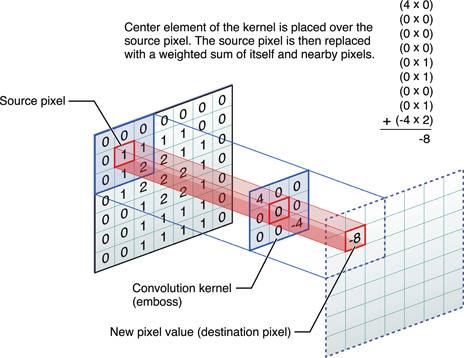
\includegraphics[width=1.0\textwidth]{./images/opencal/kernel_convolution}
        \caption{The process of determining the new value of the central cell by applying a convolution matrix to its neighborhood.}
        \label{fig:convolution}
    \end{center}
\end{figure}
Conovolution is performed multiplying the whole neighborhood of a point by a  matrix, called the \textit{kernel} of the convolution, which usually is a small square matrix of size $r$ (the most common size for kernels is $3\times 3$).
Kernels coefficients correspond to point-wise values of an arbitrary fixed continuous function, called Point Spread Functions (PSF). Figure \ref{fig:kernel_functions} depicts some of the most common PSF.

Convolution is very often used in image processing. Examples in this field are the Sobel's edge detection filter and the Gaussian Blur filters, that are shown in Figures \ref{fig:gaussian} and \ref{fig:sobel}.


\begin{figure}
    \minipage{0.65\textwidth}
    \begin{subfigure}{1.0\textwidth}
        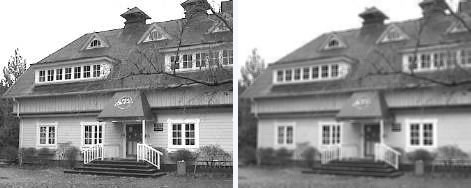
\includegraphics[width=\linewidth]{./images/opencal/gaussian_example}
        
            
    \end{subfigure}
    
    \endminipage\hfill
    \minipage{0.30\textwidth}
    \begin{subfigure}{0.9\textwidth}
        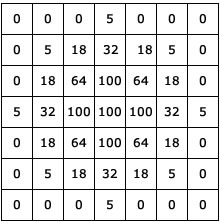
\includegraphics[width=\linewidth]{./images/opencal/conv-gaussian-blur}    
    \end{subfigure}
    \endminipage\hfill
    \caption{Gaussian Convolution filter application. The emnployed Gaussian Kernel has radius $4$.}
    \label{fig:gaussian}
\end{figure}


\begin{figure}[!htb]
    \minipage{0.65\textwidth}
    \begin{subfigure}{1.0\textwidth}
        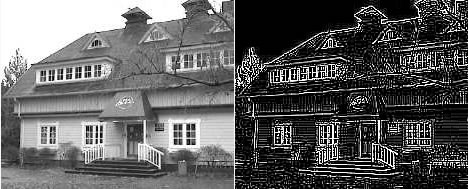
\includegraphics[width=\linewidth]{./images/opencal/sobel_example}
    \end{subfigure}
    
    \endminipage\hfill
    \minipage{0.30\textwidth}
    \begin{subfigure}{1.0\textwidth}
        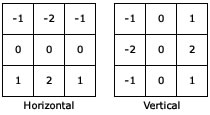
\includegraphics[width=\linewidth]{./images/opencal/conv-sobel}    
    \end{subfigure}
    \endminipage\hfill
    \caption[\textit{Sobel} edge detection filter]{\textit{Sobel} edge detection filter. The new pixel value is computed in two subsequent steps, horizontal and vertical, in order the final image to be less affected by noise.}
    \label{fig:sobel}
\end{figure}

Formally, convolution can be expressed by the following formula:
\begin{equation}
   f'_{ij} = \sum_{i'=0}^n (\sum_{j'i'=0}^m f_{(i+i')(j+j')}\times d_{ij})
   \label{eq:convolution}
\end{equation}
where 
\begin{itemize}
    \item $m,n$ are the  vertical and horizontal size of the kernel,
    \item $f_{ij}$ and $f'_{ij}$ are the old and new value of the cell at coordinate $(i,j)$,
    \item $d_{ij}$ is the value of kernel at location $(i,j)$ 
\end{itemize}

\subsubsection{Edge Handling}
It is clear from Equation \ref{eq:convolution} that kernel convolution requires values from pixels outside the domain boundaries. There are a number of ways for handling these corner cases:
\begin{description}
    \item[Wrap] \hfill \\The image is conceptually treated as it was wrapped in a toroidal shape. \texttt{OpenCAL} natively deals with toroidal domain.
    \item[Mirror] \hfill \\
    The image boundaries are mirrored at the edges, meaning that if trying to read a pixel 2 units outside the edges, the returned value is the corresponding pixel 2 unit inside the edge instead.
    \item [Crop]\hfill \\
    The final image does not contain pixel which would require values from beyond the edges. The output is smaller than the input because edges have been cropped out.
\end{description}

\subsection{Sobel Edge Detection \texttt{OpenCAL-CLUST} implementation}
\label{sec:convolutional_filters_example}
Convolutional filtering is easily implemented in \texttt{OpenCAL-CLUST} in the following steps and has been applied to the image shown in Figure \ref{fig:sobel_input}:
\begin{enumerate}
    \item Image channels are separately read by each \texttt{OpenCAL} process into \texttt{short} substates (using any image reading third part library, as \texttt{SOIL} \cite{SOIL}, for instance).
    \item A cluster file is defined for the image and shown in listing \ref{code:sobel_cluster_file}. A single node and 3 GPUs were employed in this example. Two \texttt{NVIDIA GTX980} and one \texttt{NVIDIA K40} each with an equal workload.
    \item The kernels depicted in Figure \ref{fig:sobel} are applied to each pixel of the image. \texttt{OpenCAL} kernel code is shown in Listing \ref{code:sobel_kernel}.  Boundaries are automatically handled and transferred  between devices. When devices running on different nodes need to communicate then a MPI communication takes place.
    \item The resulting image is written on disk and  shown in Figure \ref{fig:sobel_result} (optimized for book format).
\end{enumerate}

\lstset{language=[OpenCL]C,frame=tb,
    caption=\texttt{OpenCAL} Sobel edge detection filter kernel. For the sake of simplicity, filterting is performed on one color channel only., 
    label={code:sobel_kernel}, 
    basicstyle=\footnotesize\ttfamily,
    keywordstyle=\color{blue}\ttfamily,
    stringstyle=\color{red}\ttfamily,
    commentstyle=\color{green}\ttfamily,
    backgroundcolor=\color{light-gray}, 
    numbers=left,numbersep=3pt, 
    numberstyle=\tiny\ttfamily\color{gray}
%    numberstyle=\tiny
}
\begin{lstlisting}
    #define DEVICE_Q_red (0)
    
    __kernel void sobel2D_transitionFunction(__CALCL_MODEL_2D) {
    
    calclThreadCheck2D();
    int i = calclGlobalRow() + borderSize;
    int j = calclGlobalColumn();
    int KX[3][3] = {
                    {-1, 0, 1},
                    {-2, 0, 2},
                    {-1, 0, 1}};
    
    int KY[3][3] = {
                    {1, 2, 1},
                    {0, 0, 0},
                    {-1, -2, -1} };
    
    int Gx,Gy,n,k,k1;
    Gx = Gy = n = 0;
    if (j > 0 && j < calclGetColumns() - 1)
        for (k = -1; k <= 1; k++)
                for (k1 = -1; k1 <= 1; k1++) {
                Gx += calclGet2Di(MODEL_2D, DEVICE_Q_red, i + k, j + k1) *
                                                        KX[k + 1][k1 + 1];
                Gy += calclGet2Di(MODEL_2D, DEVICE_Q_red, i + k, j + k1) *
                                                        KY[k + 1][k1 + 1];
            }
    const int P = sqrt(Gx * Gx + Gy * Gy);
    //set new pixel color for red channel
    calclSet2Di(MODEL_2D, DEVICE_Q_red, i, j, P);
    return;
}

\end{lstlisting}


\lstset{language=[OpenCL]C,frame=tb,
    caption=Adopted cluster file for the Sobel filtering example. The image is decomposed equally among 3 devices. , 
    basicstyle=\footnotesize\ttfamily,
    label={code:sobel_cluster_file}
}
\begin{lstlisting}[float]
10800 21600
1
192.168.1.111 3
0 0 3600
0 1 3600
0 2 3600
\end{lstlisting}



\begin{figure}
    \minipage{1.0\textwidth}
    \begin{subfigure}{1.0\textwidth}
        \caption{Input Image}
        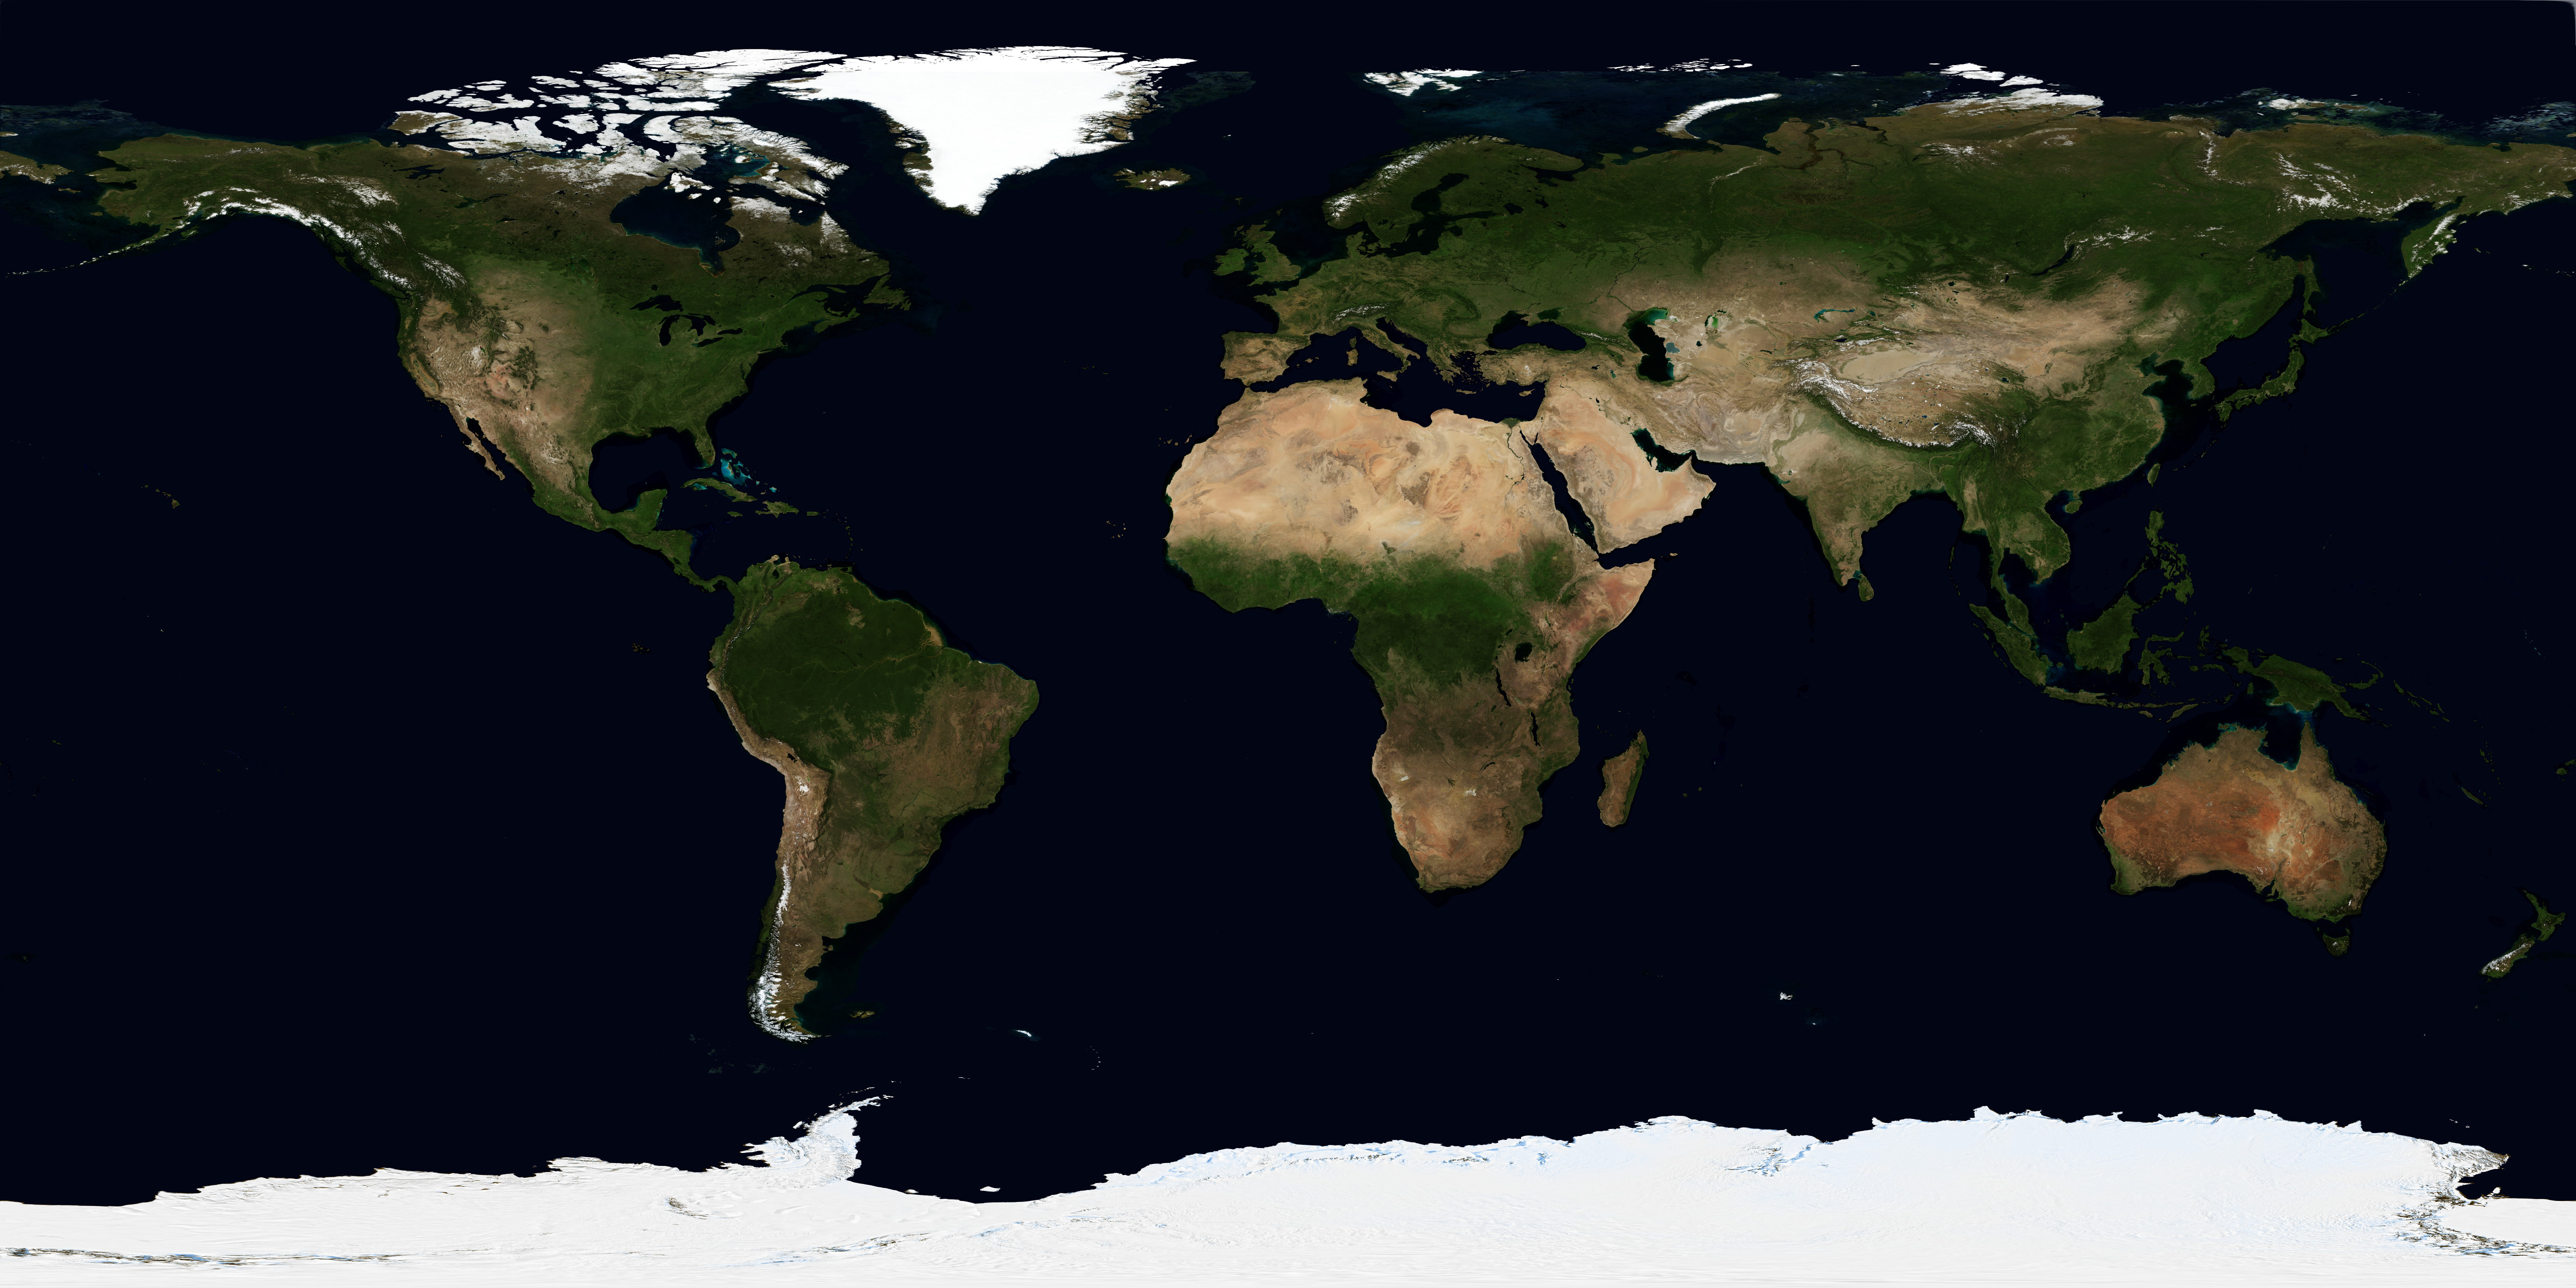
\includegraphics[width=\linewidth]{./images/opencal/sobel_input}
        \label{fig:sobel_input}
        
    \end{subfigure}    
    \endminipage\hfill \\
    \minipage{1.0\textwidth}
        \begin{subfigure}{1.0\textwidth}
        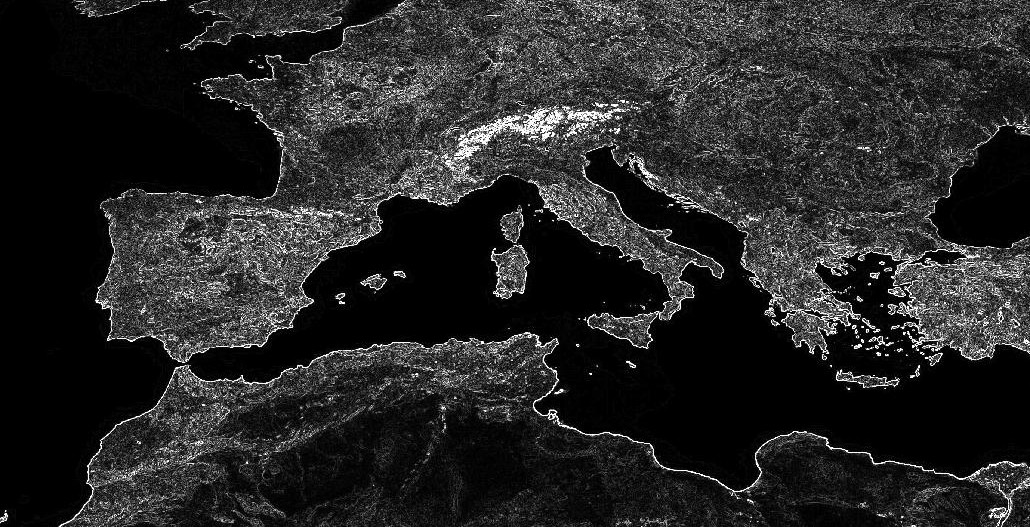
\includegraphics[width=\linewidth]{./images/opencal/sobel_output_detail}
        \label{fig:sobel_output_detail}
        \caption{Zoomed cut on Europe and North Africa of the Output Image.}
    \end{subfigure}
    \endminipage
        \caption[Input Image for the Sobel filter example shown in listing \ref{code:sobel_kernel}.]{Input Image for the Sobel filter example shown in listing \ref{code:sobel_kernel}. Image size is 233 MegaPixel $\approx 700  \si{MB}$ in \texttt{BMP} uncompressed format.}
        \label{fig:sobel_result}
\end{figure}



\subsection{SciddicaT}
\label{sec:sciddica_opencal_cluster}
This section briefly describes the \texttt{OpenCAL-CLUST} implementation of the \textit{SciddicaT} landslide model introduced in Section \ref{sec:sciddicaT_model}.
The aim of this section is to show that it is possible to deploy any model written in OpenCAL-CL to \texttt{OpenCAL-CLUST} on multiple nodes and accelerators very easily. 
The code for the implementation of sciddicaT shown in Section \ref{sec:sciddica_cl} is used in this section, with few lines added.
The additional lines take care of the definition of a cluster object, as shown in Listing \ref{code:sciddicat_configuration}, during the initialization phase, as shown in Listing \ref{code:sciddicat_initi}.
Note that in this example no configuration file is used, as to show that is possible to set up a configuration launch programmatically.

\lstset{language=[OpenCL]C,frame=tb,
    caption=[\texttt{OpenCAL-CLUST} sciddicaT Cluster definition at compile time.]{\texttt{OpenCAL-CLUST} sciddicaT Cluster defined programmatically during the \texttt{init} (see Section \ref{sec:init_finalize}) phase.}, 
    label={code:sciddicat_configuration}, 
    basicstyle=\footnotesize\ttfamily,
    keywordstyle=\color{blue}\ttfamily,
    stringstyle=\color{red}\ttfamily,
    commentstyle=\color{green}\ttfamily,
    backgroundcolor=\color{light-gray}, 
    numbers=left,numbersep=3pt, 
    numberstyle=\tiny\ttfamily\color{gray}
    %    numberstyle=\tiny
}
\begin{lstlisting}
void setUpParallelWork(Cluster& mn, const uint XDIM, const uint YDIM){
    //------node 1
    struct Node n1;
    struct Device d1_0 = {0,0,XDIM/4}; //NVIDIA  GTX980
    struct Device d1_1 = {0,1,XDIM/4}; //NVIDIA  K40
    struct Device d1_2 = {0,2,XDIM/4}; //NVIDIA  K40    
    n1.devices.push_back(d1_0);
    n1.devices.push_back(d1_1);
    n1.devices.push_back(d1_2);
    //node workload's is the sum of its devices workloads
    n1.workload = d1_0.workload+d1_1.workload+d1_2.workload;
    n1.columns=C;
    n1.offset = 0;
    mn.nodes.push_back(n1);
    
    //------node 2
    struct Node n2;
    //remainder work to this device
    struct Device d2_0 = {0,0,XDIM/4+XDIM%4};//NVIDIA K20
    n2.devices.push_back(d2_0);
    n2.workload = d2_0.workload;
    n2.columns=C;
    //n2.workload starting from n1.workload
    n2.offset = n1.workload;
    
    mn.nodes.push_back(n2);
}
\end{lstlisting}


\lstset{language=[OpenCL]C,frame=tb,
    caption=\texttt{OpenCAL-CLUST} sciddicaT model definition and launch configuration set up programmatically during the init (see Section \ref{sec:init_finalize}) phase., 
    label={code:sciddicat_initi}, 
    basicstyle=\footnotesize\ttfamily,
    keywordstyle=\color{blue}\ttfamily,
    stringstyle=\color{red}\ttfamily,
    commentstyle=\color{green}\ttfamily,
    backgroundcolor=\color{light-gray}, 
    numbers=left,numbersep=3pt, 
    numberstyle=\tiny\ttfamily\color{gray}
    %    numberstyle=\tiny
}
\begin{lstlisting}
void init( struct CALCLMultiGPU* multigpu , const Cluster* c){
Node mynode = c->nodes[rank];
auto devices = mynode.devices;
struct CALCLDeviceManager * calcl_device_manager = calclCreateManager();

calclSetNumDevice(multigpu,devices.size());
for(auto& d : devices){
    calclAddDevice(multigpu,calclGetDevice(calcl_device_manager, d.num_platform , d.num_device) ,  d.workload);
}

CALModel2D* host_CA;
host_CA = calCADef2D(mynode.workload, mynode.columns, CAL_VON_NEUMANN_NEIGHBORHOOD_2D, CAL_SPACE_TOROIDAL, CAL_OPT_ACTIVE_CELLS_NAIVE);

// Add substates
Q.f[0] = calAddSubstate2Dr(host_CA);
Q.f[1] = calAddSubstate2Dr(host_CA);
Q.f[2] = calAddSubstate2Dr(host_CA);
Q.f[3] = calAddSubstate2Dr(host_CA);
Q.z = calAddSubstate2Dr(host_CA);
Q.h = calAddSubstate2Dr(host_CA);

int my_readoffset, my_writeoffset=0;
my_readoffset = mynode.offset;
// Load configuration
calLoadSubstate2DrMulti(host_CA, Q.z, DEM_PATH,my_readoffset,my_writeoffset);
calLoadSubstate2DrMulti(host_CA, Q.h, SOURCE_PATH,my_readoffset,my_writeoffset);

// Initialization
sciddicaTSimulationInit(host_CA);
calUpdate2D(host_CA);


// Define a device-side CAs
calclMultiGPUDef2D(multigpu,host_CA,KERNEL_SRC,KERNEL_INC, 1, c->nodes.size() == 1);

// Extract kernels from program
calclAddElementaryProcessMultiGPU2D(multigpu, KERNEL_ELEM_PROC_FLOW_COMPUTATION);
calclAddElementaryProcessMultiGPU2D(multigpu, KERNEL_ELEM_PROC_WIDTH_UPDATE);

bufferEpsilonParameter = calclCreateBuffer(multigpu->context, &P.epsilon, sizeof(CALParameterr));
bufferRParameter = calclCreateBuffer(multigpu->context, &P.r, sizeof(CALParameterr));

calclAddSteeringFuncMultiGPU2D(multigpu,KERNEL_STEERING);
calclSetKernelArgMultiGPU2D(multigpu,KERNEL_ELEM_PROC_FLOW_COMPUTATION, 0,sizeof(CALCLmem), &bufferEpsilonParameter);
calclSetKernelArgMultiGPU2D(multigpu,KERNEL_ELEM_PROC_FLOW_COMPUTATION, 1, sizeof(CALCLmem), &bufferRParameter);
}
\end{lstlisting}


In this case, a configuration \texttt{Cluster} specifying two nodes and four devices in total is created. The four employed devices are: 
\begin{itemize}
    \item $2$ \textsc{nvidia} K$40$
    \item $1$ \textsc{nvidia} K$20$
    \item $1$ \textsc{nvidia} GTX$980$
\end{itemize}
(see Appendix \ref{app:tech_spec} for the technical specification of the accelerators).

The initialization phase is used here in order to allocate and initialize the library using the same approach shown in Listing \ref{code:init} (lines 7-11).

The kernel side of the application remains also the same, with the exception that boundaries cells are not considered, and are only used in read-mode. 

\section{Performance Analysis}
\label{sec:perfomance}
This section describes the computational results of \texttt{OpenCAL-CLUST} by considering the models presented in the previous sections tested on the following benchmarks:
\begin{enumerate}
    \item \textbf{Julia Set} Generation, described in Section \ref{sec:julia_math}, representing a typical compute bound application (see Section \ref{sec:julia_math}).
    \item \textbf{Convolutional Filter} application, described in Section \ref{sec:convolutional_filters}, is an example of memory bound application (see Section \ref{sec:convolutional_filters_example}).
    \item Landslide numerical model \texttt{\textbf{sciddicaT}}, introduced and formally defined in Section \ref{sec:sciddicaT_model} at page \pageref{sec:sciddicaT_model}, and is used to benchmark the performance of \texttt{OpenCAL-CLUST} on a real life computational model. Its kernels are both memory and compute bounds (see Section \ref{sec:sciddica_opencal_cluster}).
\end{enumerate}
Assessing the type of the limiting factor for performance in relatively short kernels as Julia Set generation and convolutional filter is relatively easy by considering the \textit{instruction:byte} rate of the considered kernel.
Each GPU is attached with a theoretical peak in memory and instruction throughputs\cite{Volkov:EECS-2016-143}.
Let $I$, in \si{GInst/s}, and $M$,in \si{GB/s}, be the peak instruction and memory throughput, respectively. The quantity $\frac{I}{M}$ is then called \textbf{balanced} \textit{instruction:byte} ratio. This is the number of \texttt{fp32} per byte that should be issued in order to obtain peak compute and bandwidth performance.
For example, the GPU NVIDIA K40 has a theoretical instruction throughput of $715.2$ \si{GInstr/s} and a theoretical bandwidth of $288$ \si{GB/s}. 
Its theoretical instruction throughput is computed by considering the base clock of a single core, that is $F=745$ \si{MHz} and their number, that is $N=2880$. Assuming that a \texttt{fp32} operation is completed with a latency of $L=3$ cycles then the throughput is computed as follows:
\[
    \frac{\frac{F*2880}{1000}}{3} = \frac{745*2880}{3000} = 715.2
\]

The balanced ratio for the \texttt{K40} is then:\[\frac{715.2}{288} = 2.83\]
If, compared to the \textit{balanced} ratio for the device at hand, the \textit{instruction:byte} ratio of a kernel is: 
\begin{description}
    \item[\textbf{Higher}]:\\usually means that the kernel is \textbf{instruction/compute} bound, while if it is
    \item[\textbf{Lower}]:\\usually mean that the kernel is \textbf{memory/bandwidth} bound.
\end{description}

The ratio for the Listing \ref{code:julia_set} has a value of roughly (assuming $MAXITERATION=10000$, and cost for \texttt{cl\_complex\_multiply} and \texttt{cl\_complex\_add} is equal to $2$ \texttt{fp32} instructions): $\approx 40000:1 >> 2.48$. Therefore, Listing \ref{code:julia_set} is a compute bound kernel for the $K40$ GPU.
For the same reasons we can conclude that kernel shown in Listing  \ref{code:sobel_kernel} is memory bound: its \textit{instruction:byte} ratio for is $\approx 1:1$.

SciddicaT  exposes both kind bound in its kernels. Some are memory bound, as for instance \texttt{width_update} while other are more compute intense as for instance \texttt{flow_computation}. 

\subsection{Adopted Test Hardware}
All test are executed on two computing nodes (named \textit{JPDM1} and \textit{JPDM2}, respectively) interconnected via Gigabit Ethernet.
Technical specification of both nodes can be found in Section \ref{app:tech_spec_nodes}.


\subsection{Julia Set Generation}

Fractal Generation is an example of a perfectly parallelizable problem since the computation of each point of the grid does not require any communication and does not depend on the value of any other grid points other than itself. Moreover, the granularity of the work is small, making it a good candidate for GPU acceleration.
The Julia generating function adopted is the following $z_{n+1} = z^2_n + c$ where $c=-0.391+-0.587i$. Each discrete point of the grid $(x,y)\; 0\leq x < S_x, 0\leq y < S_y$ is mapped to the complex plane using the following mapping:

\begin{align*}
    Re(z)=&\frac{3(x-\frac{S_x}{2})}{K S_x} \\
    Im(z)=&\frac{2(y-\frac{S_y}{2})}{K S_y}
\end{align*}
where $K$ is the zoom factor, $S_x$ and $S_y$ are the vertical and horizontal sizes, respectively, of the discrete computational grid.

Two domain sizes are considered:
    \begin{itemize}
        \item \textbf{small}, consisting of  $12000 \times 12000 = 144 \times 10^6$ points, $10^3$ iterations limit per step.
        \item \textbf{large}, consisting of $17000 \times 17000 = 289 \times 10^6$ points, $10^4$ iterations limit per step.
    \end{itemize}
It is worth to note that besides its much higher number of grid points, the \textit{large} domain case performs $10 \times$ more work (in a single step) per grid point than the \textit{small} case, as the number of iteration limit is increased from $10^3$ to $10^4$.

Table \ref{tab:julia_single_GPU} shows timings and speedup obtained on a single \texttt{NVIDIA K40} and \texttt{GTX980} on the \textit{small} domain.
\begin{table}
    \centering
    \caption{Timings and speedups obtained on a single \texttt{NVIDIA K40} and \texttt{GTX980} for the small dataset.}
    \label{tab:julia_single_GPU}
\begin{tabular}{@{}lll@{}}
    \toprule
    & GTX980 & K40 \\ \midrule
    \textbf{Time}$(\si{\milli\second})$    & $10908$      & $2561$   \\
    \textbf{Speedup}($\times$) & $116$      & $496$  \\
    \bottomrule
\end{tabular}
\end{table}
As expected, speedup results are extremely positive, up to $\approx 500 \times$, thanks to the great parallelizability of the problem on GPU architecture.
\begin{figure}
    
    \minipage{0.5\textwidth}
    \begin{subfigure}{1.0\textwidth}
        \caption{Fractal non-homgeneous scaling.}
        \label{fig:fractal_true_scaling}
        \includegraphics[width=1.0\textwidth]{./plots/fractal_true_scaling}
    \end{subfigure}        
    \endminipage
    \minipage{0.5\textwidth}
    
    \begin{subfigure}{1.0\textwidth}
        \caption{Fractal homogeneous work scaling}
        \label{fig:fractal_false_scaling}
        \includegraphics[width=1.0\textwidth]{./plots/fractal_false_scaling}
    \end{subfigure}
    \endminipage\hfill
    \caption[Fractal Generation speedups obtained on single and multi GPU execution.]{Fractal Generation speedups obtained on single-GPU execution (\texttt{K40}, \texttt{GTX980}) and multi-GPU execution on two devices (small dataset).
     }
    \label{fig:fractal_scaling}
\end{figure}

Table \ref{tab:julia_two_GPU}, Figures \ref{fig:julia_two_GPU} and \ref{fig:fractal_scaling} show timings and speedups of the same application on two GPUs on the \textit{small} domain. Note that since the two adopted devices  have a substantial difference in hardware (see Table \ref{tab:tech_spec_nvidia}) it is not easy to determine in advance the best workload for each of the GPU in order to obtain the best load balancing. For this reason, a number of experiments are performed in order to discover the optimal workloads for the considered GPUs and kernel.
The best speedup is obtained when only $25\%$ of the domain is assigned to the \texttt{GTX 980}.It can be seen that for this type of kernels, the $K40$ shows better performance, due to the fact that the \texttt{K40} has a higher number of processing cores and shows a better divergence management than the \texttt{GTX980}.
Moreover, it also worth to note that the Julia set kernel is highly divergent and that computational work is not homogeneously spread across the domain, as can be seen from Figure \ref{fig:fractal16k16k}. Pixels colored in blue correspond to a small number of iteration of the loop in Listing \ref{code:julia_set}, lines 23-26, while the ones colored in red to a higher number of iteration.
Note that no communication whatsoever is performed during this application since the problem is embarrassingly parallel.
The rightmost part of Figure \ref{fig:julia_two_GPU_true} (from $9000$ to $12000$) shows a weird fluctuation in the speedups, mainly due to the fact that pixels contained in rows from $1000$ to $2000$ correspond to \textit{black} ones i.e. to pixels with almost no work attached to them.
In order to show that in case of uniform work attached to each pixel the speedup curve behaves normally, a variation of Listing \ref{code:julia_set} is used and shown in Listing \ref{code:julia_set_uniform} where each execution of the kernel lasts for $1000$ iterations.
Figure \ref{fig:julia_two_GPU_false} shows that fluctuation in this case are not present.
\begin{minipage}{\linewidth}
 \lstset{language=[OpenCL]C,frame=tb,
     caption=\texttt{OpenCAL-CLUST} kernel for the generation of Julia Set. \texttt{volatile} keyword ensures that the object code for the while is emitted, 
     label={code:julia_set_uniform}, 
     basicstyle=\footnotesize\ttfamily,
     keywordstyle=\color{blue}\ttfamily,
     stringstyle=\color{red}\ttfamily,
     commentstyle=\color{green}\ttfamily,
     backgroundcolor=\color{light-gray}, 
     numbers=left,numbersep=3pt,, 
     numberstyle=\tiny\ttfamily\color{gray}
 }
 \begin{lstlisting}
 int evolveComplexPoint(cl_complex p,cl_complex c){
 int it=1;
 volatile cl_complex p1={p.x,p.y};
 while(it++ <= 1000)
     p1=juliaFunctor(p1,c);
 return 100;
 }
 \end{lstlisting}
\end{minipage}
 
%TABLE K40 -980 true and false
\begin{table}[!htb]
    \small
    \caption[Timing and speedup for the fractal generation benchmark on a \texttt{K40} and a \texttt{GTX980}.]{Timing and speedups for the fractal generation (small dataset) on a\texttt{K40} and a \texttt{GTX980}. (a) and (b) are refereed to the real case  and the uniform work scenarios, respectively. The Best speed-up case is highlighted in dark gray. The workload columns indicate the amount of rows assigned to each device.}
    \label{tab:julia_two_GPU}
    \begin{subtable}{.5\linewidth}
        \centering
        \caption{Real Fractal}
        
        \begin{tabular}{@{}CCCC@{}}
            \toprule
            \multicolumn{2}{c}{\textsc{Workload}}\\ \cline{1-2}
            \textsc{gtx980}& \textsc{K40} & \textsc{Time}$(\si{\milli\second})$ & \textsc{Speedup$(\times)$}  \\\midrule
            \rowcolor{gray!15}
            0     & 12000 & 2561  & 522.05 \\
            \rowcolor{gray!5}
            1000  & 11000 & 2520  & 530.54 \\
            \rowcolor{gray!15}
            2000  & 10000 & 2935  & 455.52 \\
            \rowcolor{gray!65}
            3000  & 9000  & 2314  & 577.77 \\
            \rowcolor{gray!15}
            4000  & 8000  & 3305  & 404.53 \\
            \rowcolor{gray!5}
            5000  & 7000  & 4458  & 299.90 \\
            \rowcolor{gray!15}
            6000  & 6000  & 6123  & 218.35 \\
            \rowcolor{gray!5}
            7000  & 5000  & 7573  & 176.54 \\
            \rowcolor{gray!15}
            8000  & 4000  & 8744  & 152.90 \\
            \rowcolor{gray!5}
            9000  & 3000  & 9669  & 138.27 \\
            \rowcolor{gray!15}
            10000 & 2000  & 10359 & 129.06 \\
            \rowcolor{gray!5}
            11000 & 1000  & 10669 & 125.31 \\
            \rowcolor{gray!15}
            12000 & 0     & 10908 & 122.57\\
            \bottomrule
        \end{tabular}
    \end{subtable}%
    \begin{subtable}{.5\linewidth}
        \centering
        \caption{Uniform number of iterations.}
        \begin{tabular}{@{}LLCC@{}}
            \toprule
            \multicolumn{2}{c}{\textsc{Workload}}\\ \cline{1-2}
            \textsc{gtx980}& \textsc{K40} & \textsc{Time}$(\si{\milli\second})$ & \textsc{Speedup$(\times)$}  \\\midrule
                \rowcolor{gray!15}
                0     & 12000 & 6039  & 193.01 \\
                \rowcolor{gray!5}
                1000  & 11000 & 5444  & 214.10 \\
                \rowcolor{gray!15}
                2000  & 10000 & 5092  & 228.91 \\
                \rowcolor{gray!65}
                3000  & 9000  & 4688  & 248.63 \\
                \rowcolor{gray!15}
                4000  & 8000  & 5043  & 231.13 \\
                \rowcolor{gray!5}
                5000  & 7000  & 6049  & 192.69 \\
                \rowcolor{gray!15}
                6000  & 6000  & 7006  & 166.37 \\
                \rowcolor{gray!5}
                7000  & 5000  & 7819  & 149.07 \\
                \rowcolor{gray!15}
                8000  & 4000  & 8771  & 132.89 \\
                \rowcolor{gray!5}
                9000  & 3000  & 9625  & 121.10 \\
                \rowcolor{gray!15}
                10000 & 2000  & 10625 & 109.70 \\
                \rowcolor{gray!5}
                11000 & 1000  & 11603 & 100.45 \\
                \rowcolor{gray!15}
                12000 & 0     & 12708 & 91.72
                 \\ 
            \bottomrule
        \end{tabular}
    \end{subtable} 
\end{table}
 

 
 
 \begin{figure}
     
     \minipage{1.0\textwidth}
     \begin{subfigure}{1.0\textwidth}
         \caption{Non Homogeneous work. High divergent code.}
         \includegraphics[width=\linewidth]{./plots/fractal12k_k40_980_true}
         \label{fig:julia_two_GPU_true}
         
     \end{subfigure}        
     \endminipage\hfill
     \minipage{1.0\textwidth}
     \vspace{5mm}
     \begin{subfigure}{1.0\textwidth}
             \caption{Homogeneous work. No thread divergence.}
         \includegraphics[width=\linewidth]{./plots/fractal12k_k40_980_false}
         \label{fig:julia_two_GPU_false}
     
     \end{subfigure}
     \endminipage\hfill
    
     \caption[Time and speed-up for the fractal generation fractal generation \textit{small} case on two different GPU: $1$ \texttt{GTX980} and $1$ \texttt{K40}.]{Time and Speed-up for the fractal generation \textit{small} case on two different GPU: $1$ \texttt{GTX980} and $1$ \texttt{K40}. The bottom and top horizontal axes indicate the amount of rows assigned to the \texttt{K40} and \texttt{GTX980}, respectively. In Figure \ref{fig:julia_two_GPU_false} are depicted time and speedup values from the modified version of the kernel \ref{code:julia_set} that force homogeneous work among the grid points.  }
     \label{fig:julia_two_GPU}
 \end{figure}

Table \ref{tab:fractal12k_980_980} and Figure \ref{fig:fractal12k_980_980} show speedup and timings for the case where two identical GPUs \texttt{GTX980} are employed. 
It is not surprising that in this case best performance are achieved when the dataset is shared in an equal manner among the two devices. However, timing and speed-up are not perfectly symmetrical in this case, since one of the GPUs is attached with the (small) overhead of performing screen rendering.

%TABLE 980 -980 true and false
\begin{table}[!htb]
\small
    \caption[Timing and speedup for the fractal generation benchmark on tow identical \texttt{GTX980}.]{Timing and speedups for the fractal generation (small dataset) on two identical \texttt{GTX980}. (a) and (b) are refereed to the real case  and the uniform work scenarios, respectively. The Best speed-up case is highlighted in dark gray.}
    \label{tab:fractal12k_980_980}
    \begin{subtable}{.5\linewidth}
        \centering
        \caption{Real Fractal}
        \begin{tabular}{@{}LLCC@{}}
            \toprule
            \multicolumn{2}{c}{\textsc{Workload}}\\ \cline{1-2}
            \textsc{gtx980}& \textsc{gtx980} & \textsc{Time}$(\si{\milli\second})$ & \textsc{Speedup$(\times)$}  \\\midrule
\rowcolor{gray!15}
0     & 12000 & 12896 & 90.38 \\
\rowcolor{gray!5}
1000  & 11000 & 11869 & 98.20 \\
\rowcolor{gray!15}
2000  & 10000 & 10968 & 106.27 \\
\rowcolor{gray!5}
3000  & 9000  & 9959  & 117.04  \\
\rowcolor{gray!15}
4000  & 8000  & 9131  & 127.65 \\
\rowcolor{gray!5}
5000  & 7000  & 8173  & 142.61 \\
\rowcolor{gray!65}
6000  & 6000  & 7088  & 164.44 \\
\rowcolor{gray!5}
7000  & 5000  & 7931  & 146.97 \\
\rowcolor{gray!15}
8000  & 4000  & 8819  & 132.17 \\
\rowcolor{gray!5}
9000  & 3000  & 9684  & 120.36 \\
\rowcolor{gray!15}
10000 & 2000  & 10629 & 109.66 \\
\rowcolor{gray!5}
11000 & 1000  & 11630 & 100.22 \\
\rowcolor{gray!15}
12000 & 0     & 12708 & 91.72 \\
            \bottomrule
        \end{tabular}
    \end{subtable}%
    \begin{subtable}{.5\linewidth}
        \centering
        \caption{Uniform number of iterations.}
        \begin{tabular}{@{}LLCC@{}}
            \toprule
            \multicolumn{2}{c}{\textsc{Workload}}\\ \cline{1-2}
            \textsc{gtx980}& \textsc{gtx980} & \textsc{Time}$(\si{\milli\second})$ & \textsc{Speedup$(\times)$}  \\\midrule
        \rowcolor{gray!15}
        0     & 12000 & 10916 & 122.48 \\
        \rowcolor{gray!5}
        1000  & 11000 & 11866 & 112.67 \\
        \rowcolor{gray!15}
        2000  & 10000 & 11595 & 115.30 \\
        \rowcolor{gray!5}
        3000  & 9000  & 10953 & 122.06 \\
        \rowcolor{gray!15}
        4000  & 8000  & 9761  & 136.97 \\
        \rowcolor{gray!5}
        5000  & 7000  & 8865  & 150.81 \\
        \rowcolor{gray!65}
        6000  & 6000  & 7132  & 187.46 \\
        \rowcolor{gray!5}
        7000  & 5000  & 7624  & 175.36 \\
        \rowcolor{gray!15}
        8000  & 4000  & 8770  & 152.45 \\
        \rowcolor{gray!5}
        9000  & 3000  & 9681  & 138.10 \\
        \rowcolor{gray!15}
        10000 & 2000  & 10341 & 129.29 \\
        \rowcolor{gray!5}
        11000 & 1000  & 10715 & 124.77 \\
        \rowcolor{gray!15}
        12000 & 0     & 10986 & 121.70 \\
            \bottomrule
        \end{tabular}
    \end{subtable} 
\end{table}

\begin{figure}
    \minipage{1.0\textwidth}
    \begin{subfigure}{1.0\textwidth}
        \caption{Non Homogeneous work. High divergent code.}
        \includegraphics[width=1.0\textwidth]{./plots/fractal12k_980_980_true}
        \label{fig:fractal12k_980_980_false}
    \end{subfigure}        
    \endminipage \hfill
    \minipage{1.0\textwidth}
     \vspace{5mm}
    \begin{subfigure}{1.0\textwidth}
        \caption{Homogeneous work. No thread divergence.}
        \includegraphics[width=1.0\textwidth]{./plots/fractal12k_980_980_false}

\label{fig:fractal12k_980_980_true}
    \end{subfigure}
    \endminipage\hfill
    \caption[Time and Speed-up for the fractal generation \textit{small} case on two GTX980.]{Time and Speed-up for the fractal generation \textit{small} case on two GTX980. The bottom and top horizontal axes indicate the amount of rows assigned to the first and second \texttt{GTX980}, respectively. In Figure \ref{fig:fractal12k_980_980_false} are depicted time and speedup values from the modified version of the kernel \ref{code:julia_set} that force homogeneous work among the grid points. Note that in this case the graph is almost perfectly symmetrical. Time in red (lower is better), speed-up in blue (higher is better).}
    \label{fig:fractal12k_980_980}
\end{figure}


Table \ref{tab:fractal12k_K40-980-980} and Figure \ref{fig:fractal12k_K40-980-980} show timing and speedup for the \textit{large} dataset that is divided among the three employed devices. In this case, the workload not assigned to the $K40$ is equally divided among the two $GTX980$ as this is the case where best performance is achieved when two identical devices are adopted, as shown in  Figure \ref{fig:fractal12k_980_980}.
\begin{figure}
    \minipage{1.0\textwidth}
    \begin{subfigure}{1.0\textwidth}
        \caption{Non homogeneous work. High divergent code. $3$ GPUs employed.}
        \includegraphics[width=1.0\textwidth]{./plots/fractal12k_K40-980-980_true}
                \label{fig:fractal12k_K40-980-980_true}
    \end{subfigure}        
    \endminipage \hfill
    \minipage{1.0\textwidth}
    \vspace{5mm}
    \begin{subfigure}{1.0\textwidth}
                \includegraphics[width=1.0\textwidth]{./plots/fractal12k_K40-980-980_false}
        \caption{Homogeneous work. No thread divergence.$3$ GPUs employed. }
        \label{fig:fractal12k_K40-980-980_false}
    \end{subfigure}
    \endminipage\hfill
\caption[Timings and Speed-up for the fractal generation \textit{large} case.]{Timings and Speed-up for the fractal generation \textit{large} case. (a) shows non-homogeneous work i.e. the real fractal, (b) the homogeneous one. Time in red (lower is better), speed-up in blue (higher is better).}
    \label{fig:fractal12k_K40-980-980}
\end{figure}
As noted, achieved speedups are good, up to to $\approx 110 \times$, when workload division is s.t. $\approx 20\%$ of the total work is shared among the two \texttt{GTX980} (see Figure \ref{fig:fractal12k_K40-980-980_true}). 
This is due to the non-homogeneous distribution of the work along the domain and to the high number of divergent threads. In fact, when homogeneity of work if forced, i.e. all threads perform the same number of iterations, the best performance are obtained assigning $\approx 40\%$  of the domain to the two \texttt{GTX980} (see Figure \ref{fig:fractal12k_K40-980-980_false}).

\begin{table}[!htb]
\footnotesize
  \caption[Timing and speedup for the fractal generation benchmark on three devices.]{Timing and speedups for the fractal generation (small dataset) on three devices: a pair of \texttt{GTX980} and a \texttt{K40}. (a) and (b) are refereed to the real case  and the uniform work scenarios, respectively. The Best speed-up case is highlighted in dark gray.}
    \label{tab:fractal12k_980_980}
    \begin{subtable}{.5\linewidth}
        \centering
        \caption{Real Fractal.}
\label{tab:fractal12k_K40-980-980}
\begin{tabular}{@{}LLLCC@{}}
    
    \toprule
\multicolumn{3}{c}{\textsc{Workload}}\\ \cline{1-3}
& \multicolumn{2}{c}{\textsc{gtx}}\\ \cline{2-3} 
\textsc{K40} &\textsc{\#1}& \textsc{\#2} & \textsc{Time}$(\si{\milli\second})$ & \textsc{Speedup$(\times)$}  \\\midrule
\rowcolor{gray!15}
16500 & 250  & 250  & 65617  & 94.8  \\
\rowcolor{gray!5}
15500 & 750  & 750  & 66438  & 93.6  \\
\rowcolor{gray!15}
14500 & 1250 & 1250 & 62685  & 99.2  \\
\rowcolor{gray!65}
13500 & 1750 & 1750 & 57851  & 107.5 \\
\rowcolor{gray!15}
12500 & 2250 & 2250 & 78570  & 79.1  \\
\rowcolor{gray!5}
11500 & 2750 & 2750 & 87098  & 71.4  \\
\rowcolor{gray!15}
10500 & 3250 & 3250 & 109818 & 56.6  \\
\rowcolor{gray!5}
9500  & 3750 & 3750 & 134713 & 46.2  \\
\rowcolor{gray!15}
8500  & 4250 & 4250 & 154125 & 40.3  \\
\rowcolor{gray!5}
7500  & 4750 & 4750 & 186840 & 33.3  \\
\rowcolor{gray!15}
6500  & 5250 & 5250 & 219067 & 28.4  \\
\rowcolor{gray!5}
5500  & 5750 & 5750 & 186668 & 33.3  \\
\rowcolor{gray!15}
4500  & 6250 & 6250 & 193661 & 32.1  \\
\rowcolor{gray!5}
3500  & 6750 & 6750 & 223505 & 27.8  \\
\rowcolor{gray!15}
2500  & 7250 & 7250 & 249335 & 24.9  \\
\rowcolor{gray!5}
1500  & 7750 & 7750 & 257837 & 24.1  \\
\rowcolor{gray!15}
500   & 8250 & 8250 & 264234 & 23.5  \\
    \bottomrule
        \end{tabular}
    \end{subtable}%
    \begin{subtable}{.5\linewidth}
    \centering
    \caption{Uniform number of iterations.}
    
    \begin{tabular}{@{}LLLCC@{}}
        \toprule
        \multicolumn{3}{c}{\textsc{Workload}}\\ \cline{1-3}
        & \multicolumn{2}{c}{\textsc{gtx}}\\ \cline{2-3} 
        \textsc{K40} &\textsc{\#1}& \textsc{\#2} & \textsc{Time}$(\si{\milli\second})$ & \textsc{Speedup$(\times)$}  \\\midrule
        \rowcolor{gray!15}
\rowcolor{gray!15}
16500 & 250  & 250  & 65617  & 94.8  \\
\rowcolor{gray!5}
15500 & 750  & 750  & 66438  & 93.6  \\
\rowcolor{gray!15}
14500 & 1250 & 1250 & 62685  & 99.2  \\
\rowcolor{gray!5}
13500 & 1750 & 1750 & 95371  & 255.8 \\
\rowcolor{gray!15}
12500 & 2250 & 2250 & 102673 & 237.6 \\
\rowcolor{gray!5}
11500 & 2750 & 2750 & 93783  & 260.2 \\
\rowcolor{gray!15}
10500 & 3250 & 3250 & 82648  & 295.2 \\
\rowcolor{gray!5}
9500  & 3750 & 3750 & 75620  & 322.7 \\
\rowcolor{gray!15}
8500  & 4250 & 4250 & 66651  & 366.1 \\
\rowcolor{gray!65}
7500  & 4750 & 4750 & 61123  & 399.2 \\
\rowcolor{gray!15}
6500  & 5250 & 5250 & 65084  & 374.9 \\
\rowcolor{gray!5}
5500  & 5750 & 5750 & 70829  & 344.5 \\
\rowcolor{gray!15}
4500  & 6250 & 6250 & 81022  & 301.1 \\
\rowcolor{gray!5}
3500  & 6750 & 6750 & 92560  & 263.6 \\
\rowcolor{gray!15}
2500  & 7250 & 7250 & 92070  & 265.0 \\
\rowcolor{gray!5}
1500  & 7750 & 7750 & 95433  & 255.7 \\
\rowcolor{gray!15}
500   & 8250 & 8250 & 108764 & 224.3
  \\
        \bottomrule
    \end{tabular}
\end{subtable}%

\end{table}

    
\subsection{Convolutional Filtering}
\label{sec:sobel_performance}
At the contrary of fractal generation, convolutional filtering is not a perfectly parallelizable problem since grid points on the boundaries requires values from grid points that reside on different GPUs. Here, the ratio of \textit{instruction:byte} is usually low (it can vary depending on the convolutional kernel adopted), meaning that the problem is low compute-intensity and latency/bandwidth bound.
Two filtering operations are taking in consideration for assessing the performance of \texttt{OpenCAL-CLUST}  on this kind of algorithm:
\begin{description}
    \item[\textbf{Sobel Edge Detection}]:\\ Described in Section \ref{sec:convolutional_filters} and which kernel is shown in Listing \ref{code:sobel_kernel},
    \item[\textbf{Gaussian Blur}]:\\ that consists of a  uniform matrix  with coefficients equal to $\frac{1}{9}$. At each step of the the application change the value of a grid point with the average of its $8$ immediate neighboring points. It has a \textit{instruction:byte} ratio $\approx 1$. See Figures \ref{fig:fractal_detail} and \ref{fig:gaussian}. Listing \ref{code:blur_kernel} shown the kernel code used for the
\end{description}
Both filters are applied on a computational grid of size $15000 \times 15000=225 \times10^6$ cells for a number of $100$ steps. The image upon which the filter are applied are generated using the \texttt{OpenCAL} fractal application described in Sections \ref{sec:julia_math}.

\begin{minipage}{\linewidth}
 \lstset{language=[OpenCL]C,frame=tb,
    caption=\texttt{OpenCAL} kernel implementing the Gaussian blur convolutional filter., 
    label={code:blur_kernel}, 
    basicstyle=\footnotesize\ttfamily,
    keywordstyle=\color{blue}\ttfamily,
    stringstyle=\color{red}\ttfamily,
    commentstyle=\color{green}\ttfamily,
    backgroundcolor=\color{light-gray}, 
    numbers=left,numbersep=3pt,, 
    numberstyle=\tiny\ttfamily\color{gray}
}
\begin{lstlisting}
int convolutional_gaussian_blur(cl_complex p,cl_complex c){
    int sum=0,n=0;
    const int sizeOfX_ =calclGetNeighbor\right oodSize();
    for(; n < sizeOfX_; ++n) 
        sum+= calclGetX2Di(MODEL_2D,DEVICE_Q_red, i, j, n);
    calclSet2Di(MODEL_2D, DEVICE_Q_red, i, j,sum/sizeOfX_);
}
\end{lstlisting}
\end{minipage}
\begin{figure}[!t]
    \begin{subfigure}[t]{0.5\textwidth}
        \centering
        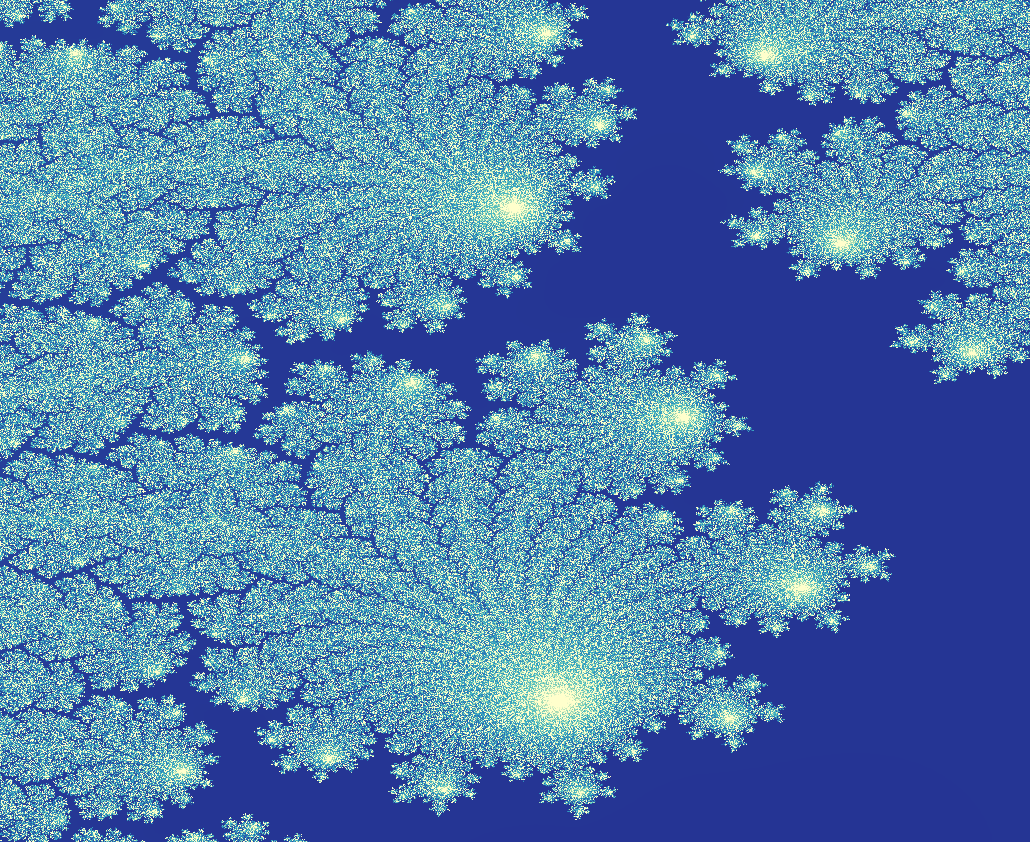
\includegraphics[width=0.9\textwidth]{./images/opencal/frattale0_detail}
        \caption{Raw detail from a rendered image of a Julia Set.}
            \label{fig:fractal_detail_raw}
    \end{subfigure}%
~
    \begin{subfigure}[t]{0.5\textwidth}
        \centering
        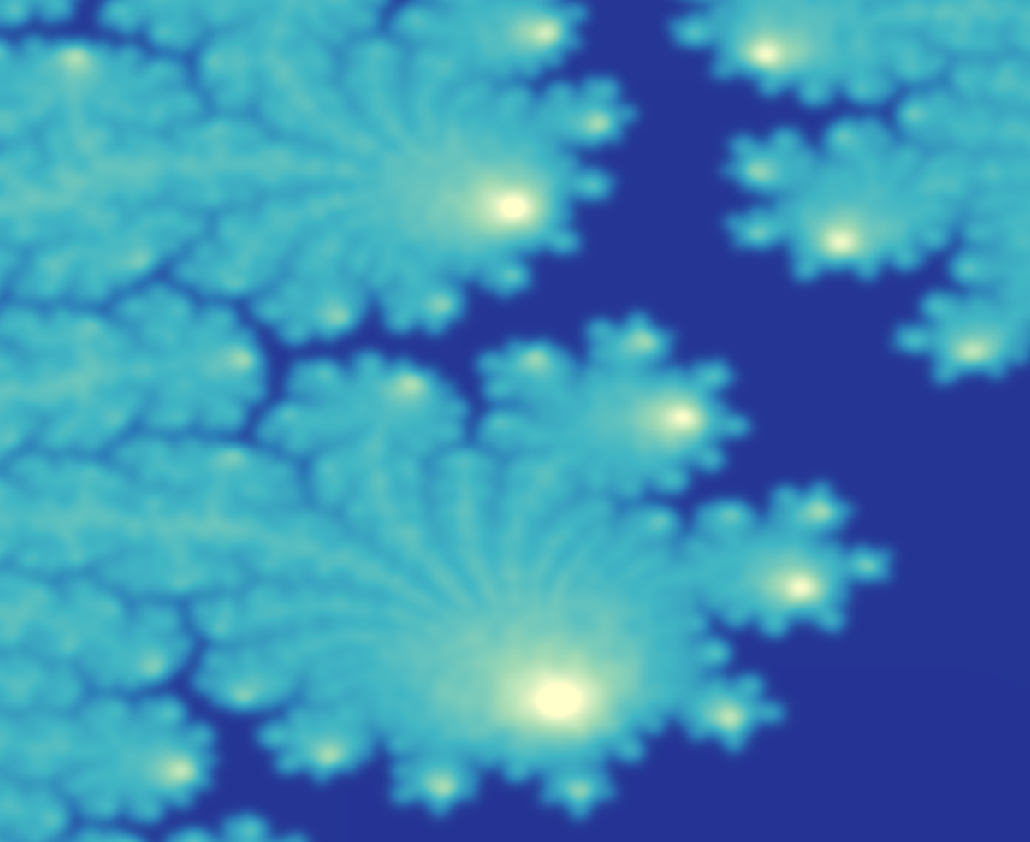
\includegraphics[width=0.9\textwidth]{./images/opencal/frattale1_blur_100_detail}
        \caption{Gaussian Blur rendered version of Figure \ref{fig:fractal_detail_raw}}
                \label{fig:fractal_detail_blur}
    \end{subfigure}
\caption[Raw and blurred detail of the of the image upon which the \texttt{OpenCAL-CLUST}  convolutional filter application is ran upon.]{Raw and blurred detail of the of the image upon which the \texttt{OpenCAL-CLUST}  convolutional filter application is ran upon. Rendering of fractals are obtained using QGIS software \cite{QGIS_software}.}
\label{fig:fractal_detail}
\end{figure}

Table \ref{tab:sobel_performance} and Figure \ref{fig:sobel_performance_charts} shows performances for the \textit{sobel} filter on two (\ref{fig:sobel_k40_980}) and three (\ref{fig:sobel_k40_980_980}) devices respectively.
Note that in this case, the disparity in performance between the \text{K40} and the \texttt{GTX980} is not evident: in-fact, best performance behavior is obtained when the domain is shared in an equal manner among the devices.
It is worth to note that the speedup scales linearly as the number of GPUs increases, as a $\approx 28 \times$ speed-up is obtained with $1$ GPU, $\approx 56 \times$ with $2$ GPUs and  $\approx 82 \times$ when $3$ devices are employed as shown in Figure \ref{fig:sobel_scaling}.


\begin{figure}

    \minipage{0.5\textwidth}
    \begin{subfigure}{1.0\textwidth}
        \caption{Blur Scaling}
        \label{fig:blur_scaling}
    \includegraphics[width=1.0\textwidth]{./plots/blur_scaling}
    \end{subfigure}        
    \endminipage
    \minipage{0.5\textwidth}

    \begin{subfigure}{1.0\textwidth}
        \caption{Sobel Scaling}
        \label{fig:sobel_scaling}
        \includegraphics[width=1.0\textwidth]{./plots/sobel_scaling}
    \end{subfigure}
    \endminipage\hfill
    \caption[]{\textbf{Blur} and \textbf{Sobel} Speed-up benchmark scales linearly with the number of GPUs. }
    \label{fig:scaling}
\end{figure}


\begin{figure}
    \minipage{1.0\textwidth}
    \begin{subfigure}{1.0\textwidth}
        \caption{Performance on $2$ GPUs: \texttt{NVIDIA K40} and $1$ \texttt{GTX980}.}
        \includegraphics[width=1.0\textwidth]{./plots/sobel_k40_980}
        \label{fig:sobel_k40_980}
    \end{subfigure}        
    \endminipage \hfill
    \minipage{1.0\textwidth}
    \vspace{5mm}
    \begin{subfigure}{1.0\textwidth}
        \includegraphics[width=1.0\textwidth]{./plots/sobel_k40_980_980}
        \caption{Performance on $3$ GPUs: \texttt{NVIDIA K40} and a pair of \texttt{GTX980}.}
        \label{fig:sobel_k40_980_980}
    \end{subfigure}
    \endminipage\hfill
    \caption[Sobel benchmark performance metrics.]{\textit{Sobel} benchmark performance metrics on two (a) and three (b) GPUs. Time in red (lower is better), speed-up in blue (higher is better).}
    \label{fig:sobel_performance_charts}
\end{figure}
\begin{table}[!htb]
    \footnotesize
    \caption{\textit{Sobel} benchmark performance metrics on two (a) and three (b) GPUs. Best speed-up case is highlighted in dark gray.}
    \label{tab:sobel_performance}
    \begin{subtable}{.5\linewidth}
        \centering
        \caption{Performance on $2$ GPUs: \texttt{NVIDIA K40} and $1$ \texttt{GTX980}.}
        
        \begin{tabular}{@{}LLCC@{}}
            \toprule
            \multicolumn{2}{c}{\textsc{Workload}}\\ \cline{1-2}
            \textsc{k40}& \textsc{gtx980} & \textsc{Time}$(\si{\milli\second})$ & \textsc{Speedup$(\times)$}  \\\midrule
            \rowcolor{gray!15}
            15000 & 0     & 97028 & 14.75 \\
            \rowcolor{gray!5}
            14000 & 1000  & 83304 & 17.18 \\
            \rowcolor{gray!15}
            13000 & 2000  & 46178 & 30.99 \\
            \rowcolor{gray!5}
            12000 & 3000  & 54814 & 26.11 \\
            \rowcolor{gray!15}
            11000 & 4000  & 41506 & 34.48 \\
            \rowcolor{gray!5}
            10000 & 5000  & 40067 & 35.72 \\
            \rowcolor{gray!15}
            9000  & 6000  & 32556 & 43.96 \\
            \rowcolor{gray!5}
            8000  & 7000  & 27314 & 52.39 \\
            \rowcolor{gray!65}
            7000  & 8000  & 26013 & 55.01 \\
            \rowcolor{gray!5}
            6000  & 9000  & 29330 & 48.79 \\
            \rowcolor{gray!15}
            5000  & 10000 & 29861 & 47.92 \\
            \rowcolor{gray!5}
            4000  & 11000 & 35657 & 40.13 \\
            \rowcolor{gray!15}
            3000  & 12000 & 38970 & 36.72 \\
            \rowcolor{gray!5}
            2000  & 13000 & 42851 & 33.39 \\
            \rowcolor{gray!15}
            1000  & 14000 & 46527 & 30.76 \\
            \rowcolor{gray!5}
            0     & 15000 & 50583 & 28.29 \\
            \bottomrule
        \end{tabular}
    \end{subtable}%
    \begin{subtable}{.5\linewidth}
        \centering
        \caption{Performance on $3$ GPUs: \texttt{NVIDIA K40} and a pair of \texttt{GTX980}.  }
        
        \begin{tabular}{@{}LLLCC@{}}
            \toprule
            \multicolumn{3}{c}{\textsc{Workload}}\\ \cline{1-3}
            & \multicolumn{2}{c}{\textsc{gtx}}\\ \cline{2-3} 
            \textsc{K40} &\textsc{\#1}& \textsc{\#2} & \textsc{Time}$(\si{\milli\second})$ & \textsc{Speedup$(\times)$}  \\\midrule
            \rowcolor{gray!15}
            14500 & 250  & 250  & 89033 & 16.07 \\
            \rowcolor{gray!5}
            13500 & 750  & 750  & 74482 & 19.21\\
            \rowcolor{gray!15}
            12500 & 1250 & 1250 & 55861 & 25.61\\
            \rowcolor{gray!5}
            11500 & 1750 & 1750 & 46666 & 30.66\\
            \rowcolor{gray!15}
            10500 & 2250 & 2250 & 39233 & 36.47\\
            \rowcolor{gray!5}
            9500  & 2750 & 2750 & 33240 & 43.05\\
            \rowcolor{gray!15}
            8500  & 3250 & 3250 & 29388 & 48.69\\
            \rowcolor{gray!5}
            7500  & 3750 & 3750 & 25364 & 56.41\\
            \rowcolor{gray!15}
            6500  & 4250 & 4250 & 22197 & 64.46\\
            \rowcolor{gray!5}
            5500  & 4750 & 4750 & 17678 & 80.94\\
            \rowcolor{gray!65}
            4500  & 5250 & 5250 & 17524 & 81.65\\
            \rowcolor{gray!5}
            3500  & 5750 & 5750 & 19415 & 73.70\\
            \rowcolor{gray!15}
            2500  & 6250 & 6250 & 21177 & 67.57\\
            \rowcolor{gray!5}
            1500  & 6750 & 6750 & 22856 & 62.60\\
            \rowcolor{gray!15}
            500   & 7250 & 7250 & 24364 & 58.73\\
            \bottomrule
        \end{tabular}
    \end{subtable}%
\end{table}

Similar results are obtained for the \textit{Gaussian blur} kernel as can be seen from Figure \ref{fig:blur_performance}.
The \textit{blur} kernel is even more memory bound than \textit{sobel}, which explains why performances are lower w.t.r to the Sobel experiments. Note that the speedup scales super-linearly as the number of GPUs increases as a $\approx 10 \times$ speed-up is obtained with $1$ GPU, $\approx 36 \times$ with $2$ GPUs and  $\approx 53 \times$ when $3$ devices are employed as shown in Figure \ref{fig:blur_scaling}.

\begin{figure}[!htb]
    \minipage{1.0\textwidth}
    \begin{subfigure}{1.0\textwidth}
        \caption{Performance on $2$ GPUs: \texttt{NVIDIA K40} and $1$ \texttt{GTX980}.}
        \label{fig:blur_k40_980}
        \includegraphics[width=1.0\textwidth]{./plots/blur_k40_980}
        
    \end{subfigure}        
    \endminipage \hfill
    \minipage{1.0\textwidth}
    \vspace{5mm}
    \begin{subfigure}{1.0\textwidth}
        \includegraphics[width=1.0\textwidth]{./plots/blur_k40_980_980}
        \caption{Performance on $3$ GPUs: \texttt{NVIDIA K40} and a pair of \texttt{GTX980}.}
        \label{fig:blur_k40_980_980}
    \end{subfigure}
    \endminipage\hfill
    \caption[\textit{Gaussinan Blur} benchmark performance metrics.]{\textit{Gaussinan Blur} benchmark performance metrics on two (a) and three (b) GPUs. Time in red (lower is better), speed-up in blue (higher is better).}
    \label{fig:blur_performance}
\end{figure}
%%%%%%%%%%%%%%%%%%%%%%%%%%%%%%%%%%%%%%%%%%%%%%%%%%%%%%%%%
\subsection{\texttt{sciddicaT}}
\texttt{sciddicaT} is an example of real life problem with both compute and memory bounds kernels. \texttt{sciddicaT} parallelization across several accelerators requires the communication of boundary cells residing on different GPUs.
Despite three benchmarks are considered for performance evaluation of \texttt{OpenCAL} as shown in Section \ref{sec:computational-results} only two benchmarks are considered here: 
\begin{description}
	\item[\textbf{Standard}]\hfil \\ the \textbf{small} standard domain of size $610 \times 496$ cells (see section \ref{sec:standard_tests})
	\item[\textbf{Computational Domain Stress Test}]\hfil \\ the \textbf{large}  domain of size $3593 \times 3730$ cells (see section \ref{sec:opencal_stress_testR})
\end{description}
Figure \ref{fig:sciddica_scaling} shows that good absolute speed-up performance, for the large dataset, are obtained when multiple devices are utilized, up to $\approx 25 \times$. It is worth to note that in this case the \texttt{GTX980} shows better performances than the $K40$ ( $9.7\times$ vs  $5.5 \times$respectively) which explain also the reason why the \texttt{sciddicaT} runs faster on a pair of \texttt{GTX980} than the case where one of them is replaced by a \texttt{K40}.
\begin{figure}[!htb]	
	\minipage{0.49\textwidth}
	\begin{subfigure}{1.0\textwidth}
		\caption{\texttt{SciddicaT} Small Dataset}
		\label{fig:sciddica_standard_scaling}
		\includegraphics[width=1.0\textwidth]{./plots/sciddicaT_standard_scaling}
	\end{subfigure}
	\endminipage
	\minipage{0.49\textwidth}
	
	\begin{subfigure}{1.0\textwidth}
		\caption{\texttt{SciddicaT} Large Dataset}
		\label{fig:sciddica_stress_scaling}
		\includegraphics[width=1.0\textwidth]{./plots/sciddicaT_scaling}
	\end{subfigure}
	\endminipage\hfill
	\caption[]{\texttt{sciddicaT} (small and large datasets) speed-up scaling as the number of GPUs is increased.}
	\label{fig:sciddica_scaling}
\end{figure}
This is mainly due to the fact that memory bounds kernels are in \texttt{sciddicaT} the ones that make up for most of the execution time, and it has been shown in Section \ref{sec:sobel_performance} that the $GTX980$ performs better executing such latency bound kernels.
Despite the good performance obtained in the \textbf{large} dataset, performance for the \textbf{standard} dataset are worse when adopting multiple devices than a single GPU configuration. The main reason is that the \textit{standard} test (see Section \ref{sec:standard_tests}) has a small number of cells ($\approx 300000$) making the efforts of further parallelization on several accelerators unnecessary since the communication overhead is dominant in this case. As it is known GPUs need a large number of threads in order to hide the intrinsic latency of the memory controller due to such latency/memory bound kernels.
Figures \ref{fig:sciddica_standard_scaling} and \ref{fig:sciddica_standard_980_k40} shows  that a negative speedups (with the respect to a \textbf{single GPU execution}) are achieved. In particular, when adopting a \texttt{K40} and a \texttt{GTX980} $\apoprox -1.5 \times$ slowdown is achieved at best.
\begin{figure}[!htb]
	\centering
	\includegraphics[width=1.0\textwidth]{./plots/sciddica_standard_k40_980}
	\caption{\texttt{sciddicaT} standard dataset on $2$ GPUs: . Time in red (lower is better), speed-up in blue (higher is better).}
	\label{fig:sciddica_standard_980_k40}
\end{figure}
Figure \ref{fig:sciddica_980_980} and \ref{fig:sciddica_k40_980} show timing and speed-ups metrics for the large dataset, for the case where a pair of \texttt{GTX980} and a \texttt{K40} and a \texttt{GTX980} are adopted, respectively. The former shows that slightly super-linear speedup is achieved when an equal amount of work is assigned to each device while the latter configuration achieves best performance when only $\approx 30\%$ of the domain is assigned to the \texttt{K40} reaching a peak of $\approx 5 \times$ speedup.
Figure \ref{fig:sciddica_k40_980_980} shows timing and speed-up in the case where $3$ GPUs are adopted. In this case best performance are achieved when only $\approx 15\%$ of the domain is assigned to the \texttt{K40} obtaining a speedup of  $\approx 25 \times$.
\begin{figure}
	\minipage{0.81\textwidth}
	\begin{subfigure}{1.0\textwidth}
	
		\includegraphics[width=1.0\textwidth]{./plots/sciddica_k40_980}
			\caption{Performance on $2$ GPUs: \texttt{NVIDIA K40} and $1$ \texttt{GTX980}.}
		\label{fig:sciddica_k40_980}
	\end{subfigure}        
	\endminipage \hfill
	\minipage{0.81\textwidth}

	\begin{subfigure}{1.0\textwidth}
		\includegraphics[width=1.0\textwidth]{./plots/sciddica_980_980}
		\caption{Performance on $2$ GPUs: a pair of \texttt{NVIDIA GTX980}.}
		\label{fig:sciddica_980_980}
	\end{subfigure}
	\endminipage\hfill
	\minipage{0.81\textwidth}
	\begin{subfigure}{1.0\textwidth}
		\includegraphics[width=1.0\textwidth]{./plots/sciddica_k40_980_980}
		\caption[\texttt{sciddicaT} performance on $3$ GPUs.]{\texttt{sciddicaT} performance on $3$ GPUs: a pair of \texttt{NVIDIA GTX980} and a \texttt{NVIDIA K40}.}
		\label{fig:sciddica_k40_980_980}
	\end{subfigure}
	\endminipage\hfill
	
	\caption[\texttt{sciddicaT} benchmark performance metrics.]{\texttt{sciddicaT} benchmark performance metrics on a \texttt{NVIDIA K40} and \texttt{NVIDIA GTX980} (a) and on  a pair of \texttt{NVIDIA GTX980} (b) GPUs. Time in red (lower is better), speed-up in blue (higher is better).}
	\label{fig:sciddica_performance}
\end{figure}

\subsection{Conclusion and Future Works}
This chapter introduced the preliminary implementation of the distributed memory and multi-GPU  version of \texttt{OpenCAL}: \texttt{OpenCAL-CLUST}.
It has been shown that it allows deploying numerical application on regular grid on machines composed by several computational nodes interconnected by network each armed with multiple accelerators. Thanks to the adoption of \texttt{OpenCL}, different kind of accelerators can be employed seamlessy.
The performance benchmarks that have been used to test \texttt{OpenCAL-CLUST} ( Section \ref{sec:perfomance}) show that it effectively use the computational power of multiple device in order to speedup the computation.

As regarding future developments, \texttt{OpenCAL-CLUST} will be  extended allowing domain decomposition on multiple dimensions. As shown in Section \ref{sec:domain_decomposition}, decomposing the domain on a single dimension is not always optimal. The programmer would be able to decompose the domain multidimensional cubic portions and assign one to each available device.
Another important issue that will be addressed is that the current implementation serialize communications at each step execution. 
This might not be optimal in cases where boundaries grid cells between two devices or nodes do not change. The communication of such cells can be avoided. This mechanism can be accomplished by performing boundaries exchange only if there is a relevant update (using the so called \textit{dirty-bits}). 


